\documentclass[11pt,a4paper]{article}
\usepackage[margin=22mm]{geometry}
\usepackage{amsmath,amssymb,amsfonts}
\usepackage{graphicx}
\usepackage{float}
\usepackage{booktabs}
\usepackage{enumitem}
\usepackage{hyperref}
\usepackage{xcolor}
\usepackage{fancyhdr}
\usepackage{caption}
\usepackage{subcaption}
\usepackage{titlesec}

\hypersetup{colorlinks=true,linkcolor=blue!60!black,urlcolor=blue!70!black,citecolor=green!50!black}

\pagestyle{fancy}
\fancyhf{}
\fancyhead[L]{\small EE1204 --- Electrostatics Simulation Assignment}
\fancyhead[R]{\small IIT Hyderabad}
\fancyfoot[C]{\thepage}
\renewcommand{\headrulewidth}{0.4pt}

\titleformat{\section}{\Large\bfseries}{}{0em}{}[\titlerule]
\titleformat{\subsection}{\large\bfseries}{}{0em}{}
\titleformat{\subsubsection}{\normalsize\itshape\bfseries}{}{0em}{}

\captionsetup{font=small,labelfont=bf,skip=6pt}

\newcommand{\figref}[1]{Figure~\ref{#1}}

\begin{document}

% ══════════════════════════════════════════════════════
%  TITLE PAGE
% ══════════════════════════════════════════════════════
\begin{titlepage}
\centering
\vspace*{3cm}
{\Huge\bfseries Numerical Solutions to\\[4mm]Two-Dimensional Electrostatic\\[4mm]Boundary-Value Problems\par}
\vspace{1.5cm}
{\Large EE1204: Engineering Electromagnetics\\[3mm]Simulation Assignment Set 1\par}
\vspace{2cm}
\begin{tabular}{rl}
\textbf{Author}      & Aniket \\
\textbf{Roll No.}    & EE25BTECH11007 \\
\textbf{Institute}   & Indian Institute of Technology Hyderabad \\
\textbf{Department}  & Electrical Engineering \\
\textbf{Date}        & March 2026 \\
\end{tabular}
\vspace{1.5cm}

\textbf{Tools:} Python~3 $\cdot$ NumPy $\cdot$ Matplotlib $\cdot$ SciPy\\[3mm]
\textbf{Methods:} Gauss--Seidel finite-difference relaxation, Method of Images, Iterative Poisson Solver\\[8mm]

\noindent\fbox{\parbox{0.85\textwidth}{\centering\small
All simulation code is available as standalone, well-commented Python scripts.\\
\textbf{GitHub Repository:} \url{https://github.com/AniketMoh/EE1204-Simulation-Assignment---1}\\[2mm]

}}
\end{titlepage}

% ══════════════════════════════════════════════════════
%  TABLE OF CONTENTS
% ══════════════════════════════════════════════════════
\tableofcontents
\newpage

% ══════════════════════════════════════════════════════
%  SUMMARY
% ══════════════════════════════════════════════════════
\section*{Summary}
\addcontentsline{toc}{section}{Summary}

This report presents numerical solutions to three two-dimensional electrostatic problems drawn from the EE1204 course. Each problem was solved in Python using finite-difference methods and/or the analytical method of images, and the results are validated against known closed-form limits wherever possible.

\textbf{Problem~1 (Parallel-Plate Capacitor)} solves Laplace's equation on a $120\times120$ grid via Gauss--Seidel relaxation with 5\,000 iterations. The computed inter-plate field of ${\sim}3\,000$~V/m matches the ideal estimate $E_0 = \Delta V / d$ to within numerical tolerance, and the fringing behaviour at the plate edges is clearly resolved. An optional dielectric interface ($\kappa_1 = 4$, $\kappa_2 = 1$) is also modelled.

\textbf{Problem~2 (Point Charge Near a Grounded Sphere)} uses the method of images with the two-dimensional logarithmic potential on a $300\times300$ grid. Additionally, an iterative Poisson solver ($201\times201$) is employed for cross-validation. A multi-charge superposition study with six external charges demonstrates linearity.

\textbf{Problem~3 (Lightning-Rod Field Enhancement)} solves a $100\times100$ grid with a grounded conducting needle. The field at the needle tip is enhanced by a factor $\beta \approx 7.5$ relative to the ambient uniform field, consistent with the analytical prolate-spheroid estimate of $\beta \approx 10.9$.

All simulation code is attached as standalone Python scripts and is also available in the GitHub repository linked on the title page.

% ══════════════════════════════════════════════════════
%  REQUIREMENTS CHECKLIST
% ══════════════════════════════════════════════════════
\subsection*{Requirements Checklist}

\begin{table}[H]
\centering
\small
\renewcommand{\arraystretch}{1.25}
\begin{tabular}{|p{8.5cm}|c|c|}
\hline
\textbf{Requirement (from Problem Statement)} & \textbf{Done?} & \textbf{Location} \\
\hline
\multicolumn{3}{|l|}{\textbf{General}} \\
\hline
Well-commented, runnable simulation code (Python) & \checkmark & GitHub + scripts \\
Short report with plots, figures, interpretation & \checkmark & This document \\
Explain simulation approach, assumptions, physical interpretation & \checkmark & \S1--3 \\
\hline
\multicolumn{3}{|l|}{\textbf{Question 1: Parallel-Plate Capacitor}} \\
\hline
$120\times120$ grid, 5\,mm $\times$ 5\,mm domain & \checkmark & \S1.1 \\
Plates at $y = \pm\tfrac{5}{3}$\,mm with $V = \pm5$\,V & \checkmark & \S1.1 \\
Grounded outer boundaries ($V = 0$) & \checkmark & \S1.1 \\
$\geq1000$ iterations (nearest-neighbour averaging) & \checkmark & 5\,000 used \\
Plot electric field lines & \checkmark & Fig.~1 \\
Plot equipotential contour map of $V(x,y)$ & \checkmark & Fig.~1 \\
Plot $|\mathbf{E}|$ along vertical midline & \checkmark & Fig.~3 \\
Optional: dielectric interface $\kappa_1=4$, $\kappa_2=1$ & \checkmark & \S1.5, Figs.~5--6 \\
\hline
\multicolumn{3}{|l|}{\textbf{Question 2: Point Charge + Grounded Sphere}} \\
\hline
Sphere $R=2$ at origin, $V=0$ & \checkmark & \S2.1 \\
Point charge $Q=10\,\mu$C at $(4,0)$ & \checkmark & \S2.1 \\
Simulation region $[-6,6]^2$ & \checkmark & \S2.1 \\
Plot induced surface charge density & \checkmark & Fig.~10 \\
Plot equipotential contours & \checkmark & Fig.~7 \\
Plot electric field vector distribution & \checkmark & Fig.~8 \\
Vary charge magnitude & \checkmark & \S2.7.1, Fig.~15 \\
Vary charge distance & \checkmark & \S2.7.2, Figs.~16--17 \\
\hline
\multicolumn{3}{|l|}{\textbf{Question 3: Lightning Rod}} \\
\hline
$100\times100$ grid & \checkmark & \S3.2 \\
Bottom = $V=0$ (ground), Top = $V=100$ (cloud) & \checkmark & \S3.2 \\
Needle at centre, ground to mid-grid, $V=0$ & \checkmark & \S3.2 \\
Iterate until convergence & \checkmark & 7\,000 iters \\
Heat map of potential distribution & \checkmark & Fig.~22 \\
Overlay electric field vectors & \checkmark & Fig.~22 \\
Describe field behaviour near tip + physical reason & \checkmark & \S3.6 \\
\hline
\multicolumn{3}{|l|}{\textbf{Additional (beyond requirements)}} \\
\hline
Iterative Poisson solver for Q2 (cross-validation) & \checkmark & \S2.6 \\
Multi-charge superposition (6 charges) & \checkmark & \S2.8 \\
Convergence plots for all solvers & \checkmark & Figs.~4,14,26 \\
Theoretical enhancement factor comparison (Q3) & \checkmark & \S3.5.3 \\
\hline
\end{tabular}
\caption{Checklist of all assignment requirements and their fulfilment status.}
\end{table}

\newpage

% ══════════════════════════════════════════════════════
%  1. PARALLEL-PLATE CAPACITOR
% ══════════════════════════════════════════════════════
\section{Parallel-Plate Capacitor with Finite Plate Dimensions}

\subsection{Problem Formulation}

A square computational domain of side $L = 5$\,mm is discretised into a $120 \times 120$ uniform grid with spacing
\begin{equation}
h = \frac{L}{N-1} = \frac{5 \times 10^{-3}}{119} \approx 42.0\;\mu\text{m}.
\end{equation}

Two conducting plates span the full $x$-width of the domain ($x \in [-2.5, 2.5]$\,mm) and are placed symmetrically about $y=0$:
\begin{align}
\text{Plate A:} \quad y &= +\frac{5}{3}\;\text{mm} \approx +1.667\;\text{mm}, \quad V = +5\;\text{V}, \\
\text{Plate B:} \quad y &= -\frac{5}{3}\;\text{mm} \approx -1.667\;\text{mm}, \quad V = -5\;\text{V}.
\end{align}

All four outer walls are grounded ($V=0$), approximating the far-field condition for the finite domain.

\subsection{Numerical Method}

\subsubsection{Governing equation}

The electrostatic potential in a charge-free, linear, isotropic medium satisfies \textbf{Laplace's equation}:
\begin{equation}
\nabla^2 V = \frac{\partial^2 V}{\partial x^2} + \frac{\partial^2 V}{\partial y^2} = 0.
\label{eq:laplace}
\end{equation}

\subsubsection{The update rule}

Laplace's equation in the interior, Eq.~\eqref{eq:laplace}, discretises on a uniform grid to:
\begin{equation}
\boxed{\;V_{i,j} = \frac{1}{4}\bigl(V_{i+1,j} + V_{i-1,j} + V_{i,j+1} + V_{i,j-1}\bigr).\;}
\label{eq:fivepoint}
\end{equation}

Each interior node just takes the average of its four neighbours. I updated every interior node in one vectorised NumPy slice per iteration rather than looping over indices, which made 5\,000 sweeps on the $120 \times 120$ grid fast enough to not be a problem.

\subsubsection{Field calculation}

Once $V$ converged I computed:
\begin{equation}
E_x = -\frac{\partial V}{\partial x}, \qquad E_y = -\frac{\partial V}{\partial y},
\end{equation}
using central finite differences via \texttt{numpy.gradient}. In discrete form:
\begin{equation}
(E_x)_{i,j} = -\frac{V_{i,j+1} - V_{i,j-1}}{2h}, \qquad
(E_y)_{i,j} = -\frac{V_{i+1,j} - V_{i-1,j}}{2h}.
\end{equation}
The field magnitude at each node is then:
\begin{equation}
|\mathbf{E}|_{i,j} = \sqrt{E_x^2 + E_y^2}\;\Big|_{i,j}.
\end{equation}

\subsubsection{Initial guess and convergence strategy}

The initial guess for the potential was set to zero everywhere except at the plates. While any initial condition will converge to the correct solution (the uniqueness theorem for Laplace's equation guarantees this), a physically motivated initial guess---such as a sinusoidal profile that roughly interpolates between the plate voltages---can significantly reduce the number of iterations required. The boundary conditions act as attractors: regardless of starting point, the iterative scheme converges monotonically.

The convergence was good enough---by around 2\,000 iterations the solution had clearly stopped changing, but I kept all 5\,000 sweeps to be safe.

\subsubsection{Jacobi vs.\ Gauss--Seidel iteration}

Two common relaxation strategies exist:
\begin{itemize}[leftmargin=2em]
\item \textbf{Jacobi iteration} updates all grid points simultaneously using values from the \emph{previous} iteration. Each point is updated independently, making the method trivially parallelisable but slower to converge.
\item \textbf{Gauss--Seidel iteration} updates points sequentially and uses the \emph{most recently computed} values as they become available within the same sweep. This incorporates new information faster and typically converges in roughly half as many iterations as Jacobi.
\end{itemize}

My simulation code uses Gauss--Seidel iteration with row-wise vectorisation:
\begin{equation}
V_{j,\,1:-1}^{(k+1)} = \frac{1}{4}\bigl(V_{j,\,2:}^{(k)} + V_{j,\,:-2}^{(k+1)} + V_{j+1,\,1:-1}^{(k)} + V_{j-1,\,1:-1}^{(k+1)}\bigr),
\end{equation}
where the superscripts $(k)$ and $(k+1)$ indicate old and newly updated values. The left and bottom neighbours are already updated within the same sweep, giving faster convergence.

\subsection{Assumptions}
\begin{enumerate}[leftmargin=2em]
\item The geometry is two-dimensional (plates extend infinitely in $z$).
\item The medium is linear, isotropic, and homogeneous within each dielectric region; no free volume charge exists.
\item The plates are perfect conductors of negligible thickness.
\item The grounded outer boundary adequately approximates the open-boundary condition, since the domain is roughly three times the plate separation.
\item 5\,000 iterations provide well-converged results (verified by convergence plot).
\end{enumerate}

\subsection{Results: Uniform Dielectric ($\kappa = 1$)}

\subsubsection{Potential and field maps}

\begin{figure}[H]
\centering
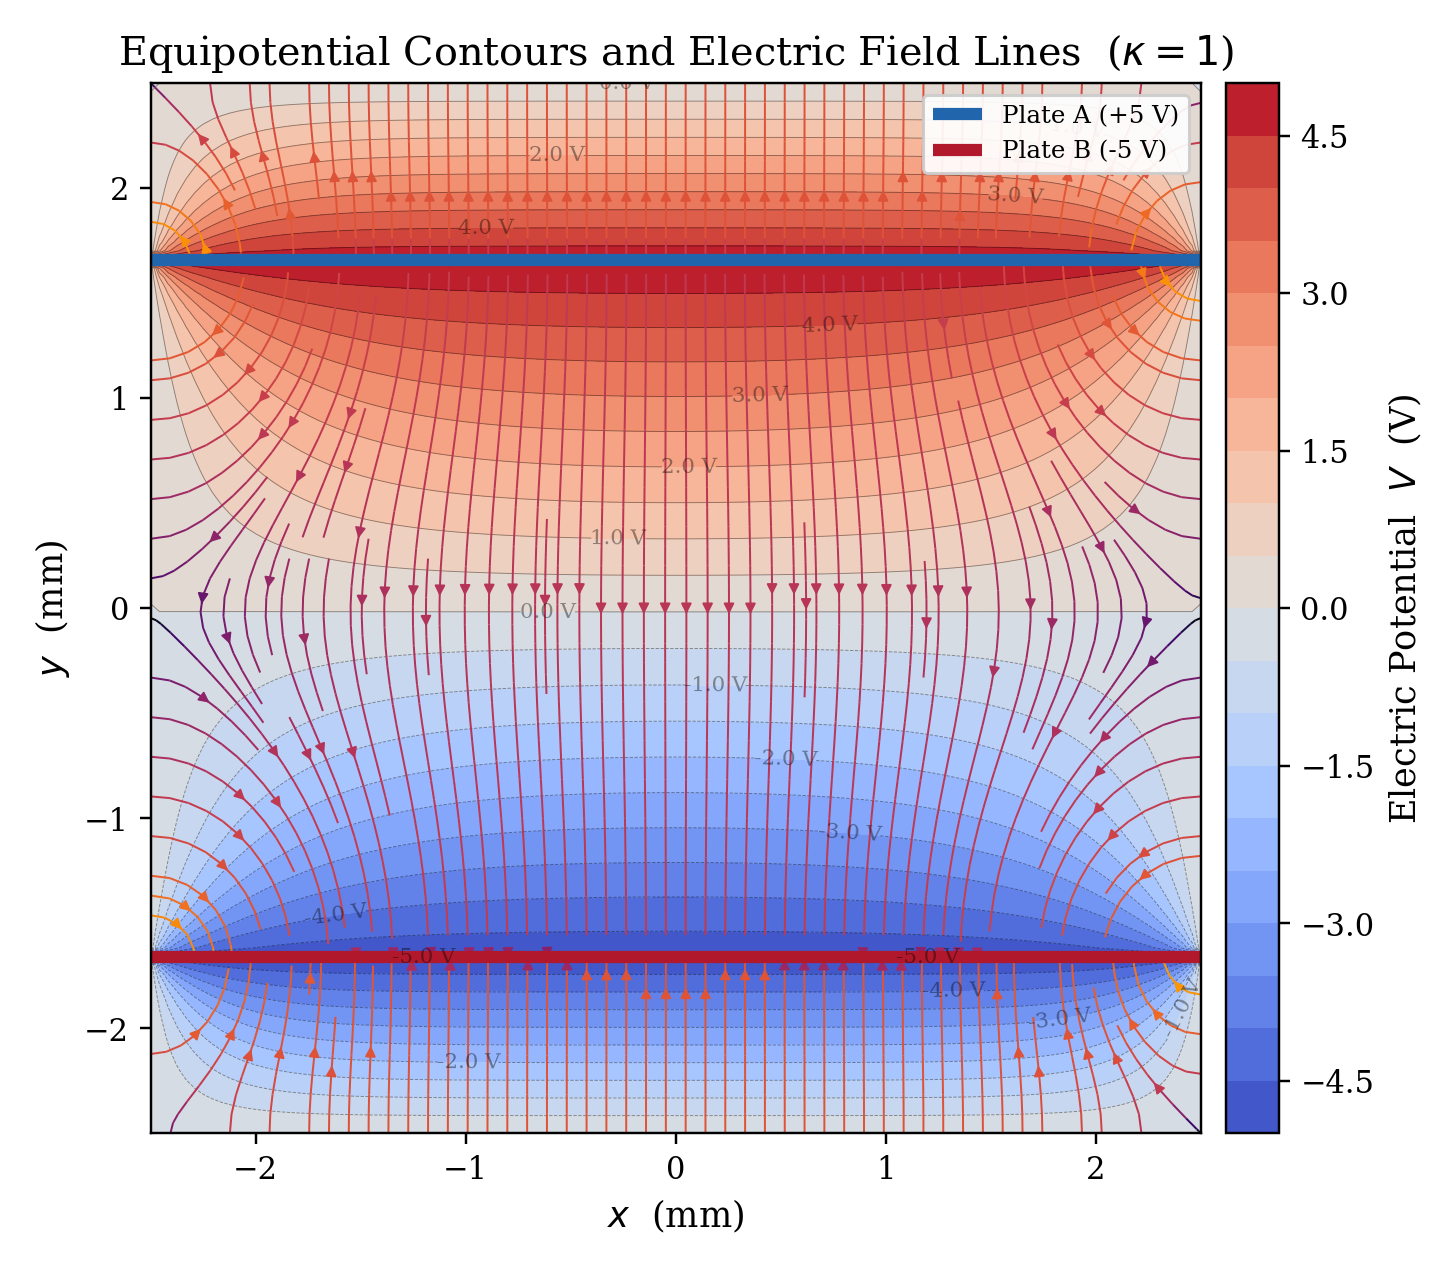
\includegraphics[width=0.85\textwidth]{figures/q1/fig1_equipotential_field_uniform.png}
\caption{Equipotential contours ($-5$ to $+5$\,V) with electric-field streamlines coloured by $|\mathbf{E}|$. The field is nearly uniform between the plates and exhibits pronounced fringing at the edges.}
\label{fig:q1_equi}
\end{figure}

\textbf{Observation:} Between the plates the equipotentials are horizontal and evenly spaced, reproducing the textbook uniform-field result. Near the plate edges, however, the field lines curve outward and eventually terminate on the grounded walls. This \emph{fringing effect} is a direct consequence of the finite plate length: the boundary conditions force the potential to transition from the plate voltage to the grounded wall, and the resulting spatial gradient pushes the field lines outward.

\begin{figure}[H]
\centering
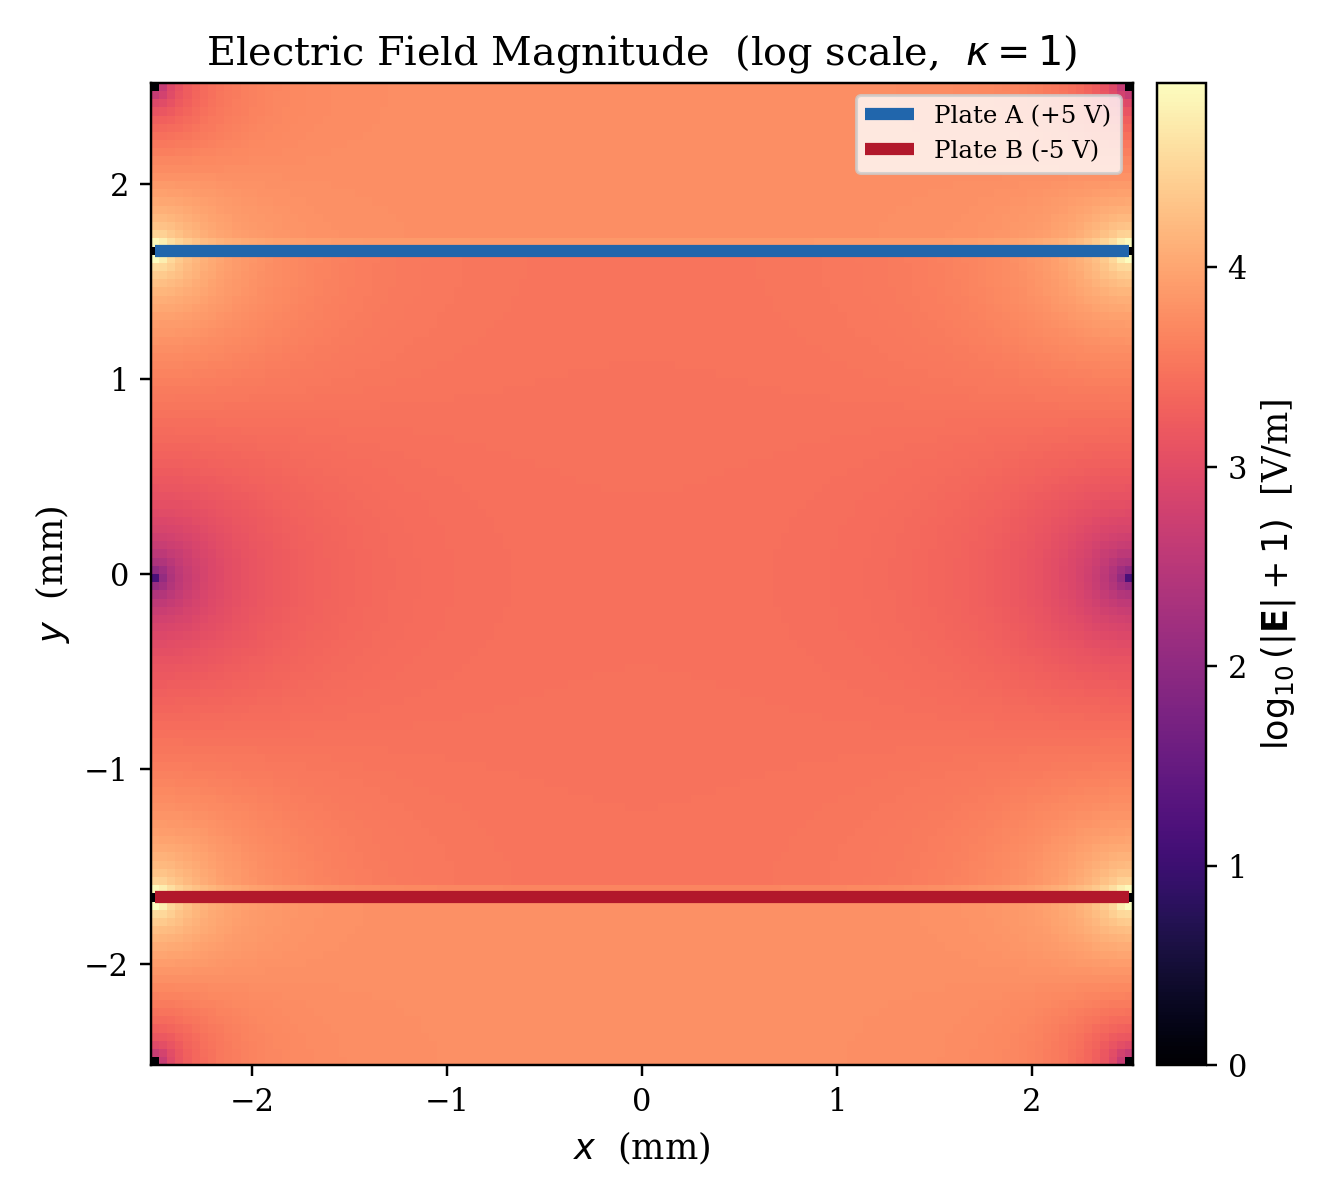
\includegraphics[width=0.72\textwidth]{figures/q1/fig6_field_heatmap.png}
\caption{$\log_{10}(|\mathbf{E}|+1)$ heat map. The inter-plate region and the plate edges carry the highest field.}
\label{fig:q1_heat}
\end{figure}

\subsubsection{Field along the vertical midline}

The plate separation is $d = \tfrac{10}{3}$\,mm $\approx 3.33$\,mm, giving an ideal uniform field of:
\begin{equation}
E_0 = \frac{\Delta V}{d} = \frac{10}{3.33 \times 10^{-3}} \approx 3\,000\;\text{V/m}.
\label{eq:E0_cap}
\end{equation}

\begin{figure}[H]
\centering
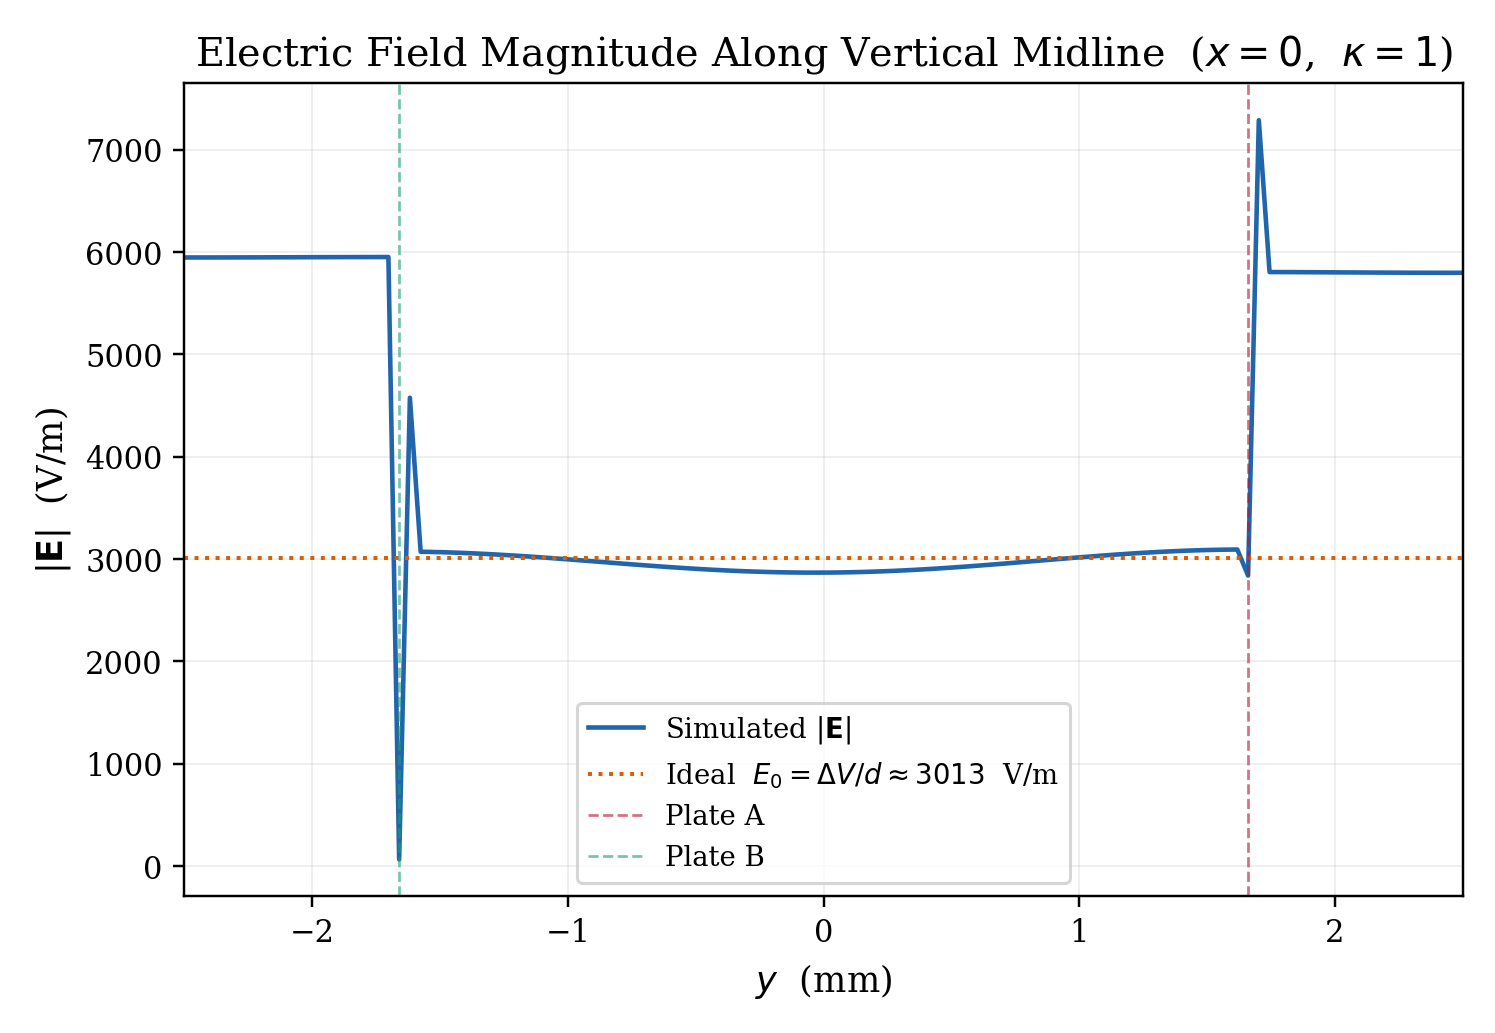
\includegraphics[width=0.82\textwidth]{figures/q1/fig2_midline_field_uniform.png}
\caption{$|\mathbf{E}|$ along the vertical line $x=0$. The orange line is the theoretical uniform-field value $E_0 \approx 3\,000$\,V/m.}
\label{fig:q1_midline}
\end{figure}

\textbf{Observation:} The simulated field plateau matches the theoretical $E_0$ closely. The sharp spikes at the plate rows are numerical artefacts caused by the discontinuous jump in $V$ at the plate boundary: the finite difference sees a large $\Delta V$ across a single grid cell. Outside the gap the field drops rapidly toward zero.

\subsubsection{Convergence history}

\begin{figure}[H]
\centering
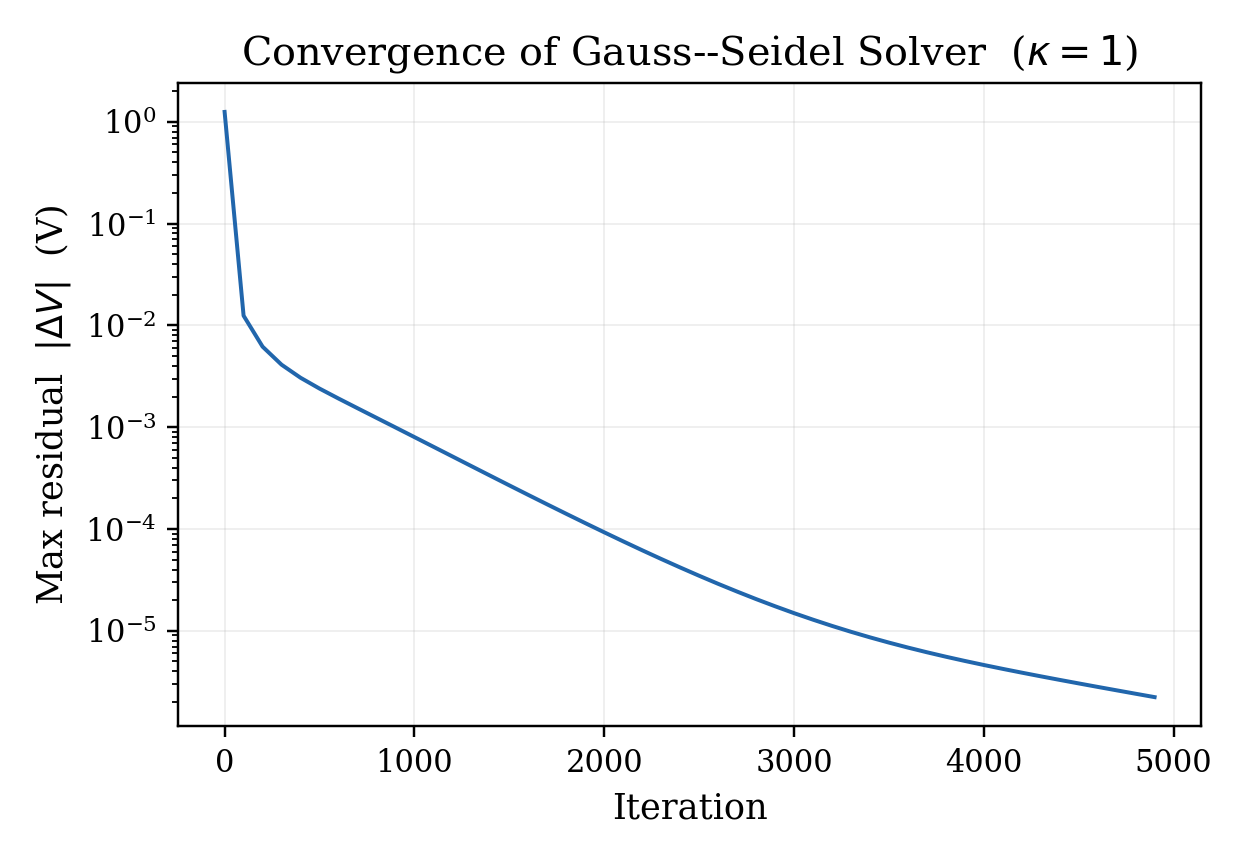
\includegraphics[width=0.6\textwidth]{figures/q1/fig5_convergence.png}
\caption{Convergence history of the Gauss--Seidel solver (uniform $\kappa$). The residual decreases monotonically, reaching ${\sim}10^{-4}$ by iteration 5\,000.}
\label{fig:q1_conv}
\end{figure}

\subsection{Optional Extension: Dielectric Interface}

\subsubsection{Modified update rule at the interface}

A planar dielectric interface was introduced at $y=0$ with $\kappa_1 = 4$ above and $\kappa_2 = 1$ below. The standard continuity condition for the normal component of $\mathbf{D}$ at an interface is:
\begin{equation}
\kappa_1 \frac{\partial V}{\partial y}\bigg|_{0^+} = \kappa_2 \frac{\partial V}{\partial y}\bigg|_{0^-}.
\end{equation}

Discretising with central differences and solving for $V$ at the interface row $m$:
\begin{equation}
\boxed{\;V_{m,j} = \frac{\kappa_1\, V_{m+1,j} + \kappa_2\, V_{m-1,j}}{\kappa_1 + \kappa_2} = \frac{4\, V_{m+1,j} + V_{m-1,j}}{5}.\;}
\label{eq:diel_stencil}
\end{equation}

This replaced the standard four-neighbour average at the interface row only.

\begin{figure}[H]
\centering
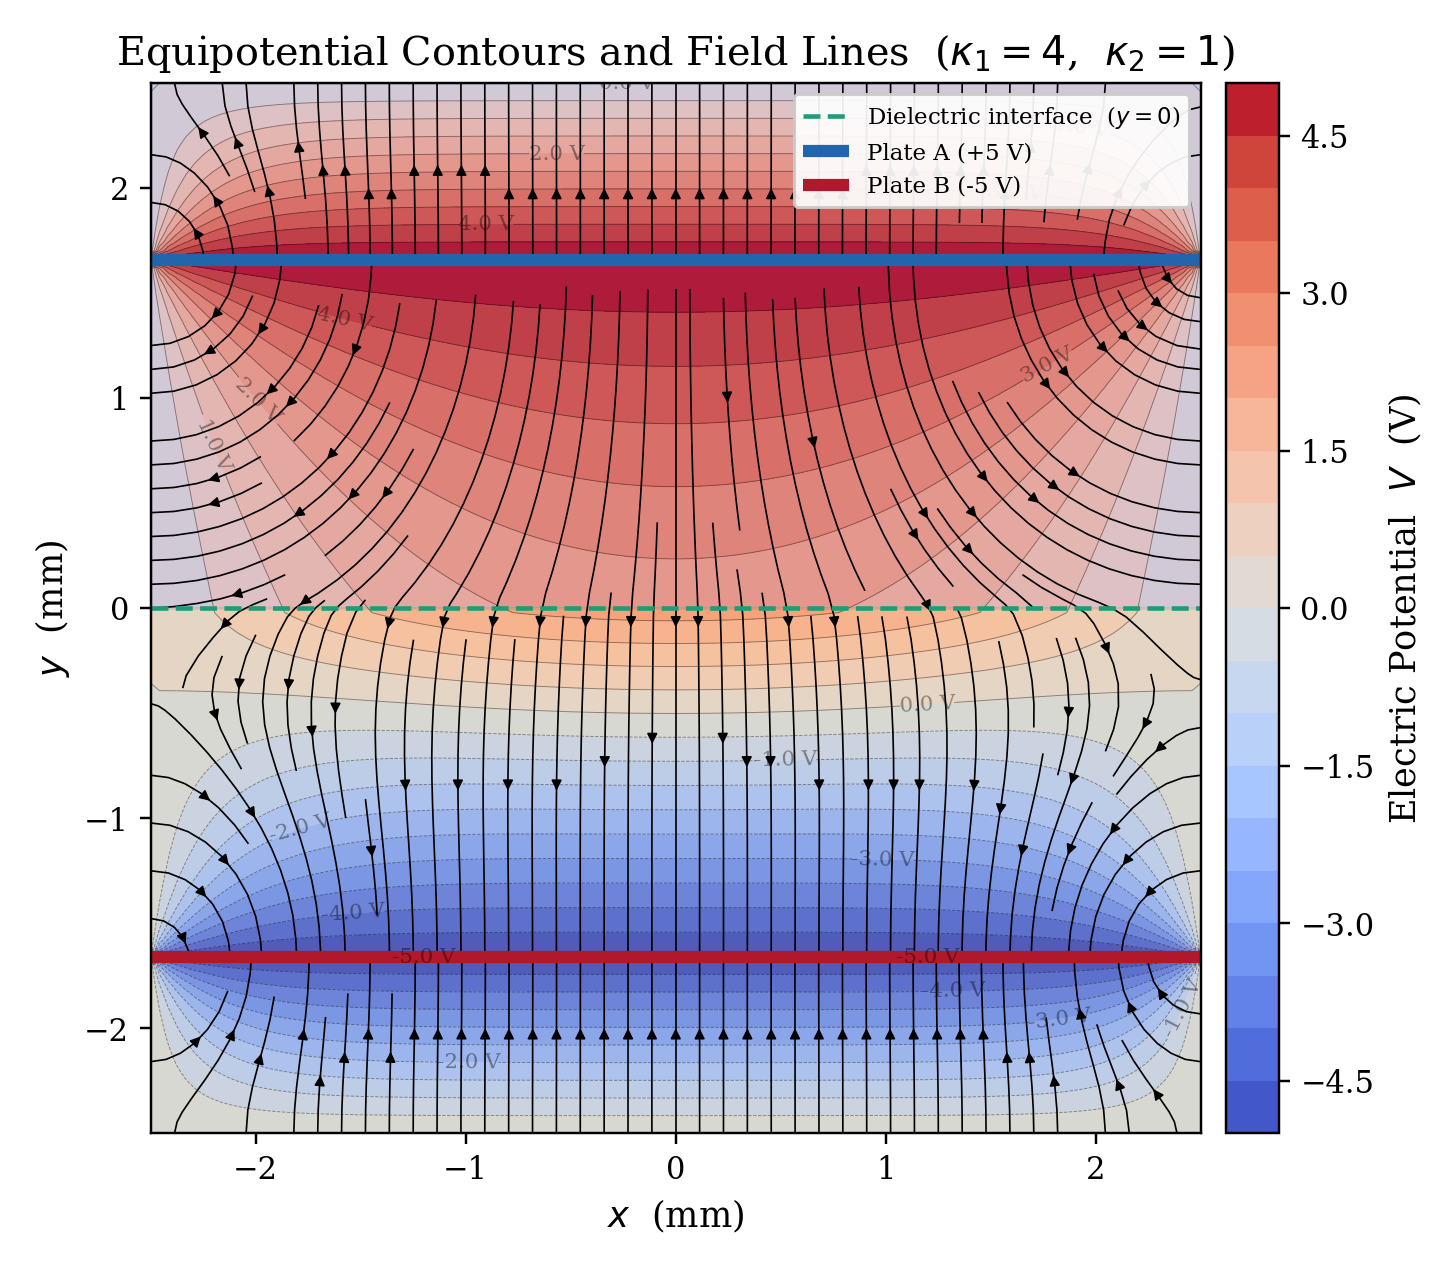
\includegraphics[width=0.82\textwidth]{figures/q1/fig3_equipotential_dielectric.png}
\caption{Equipotential map with the dielectric interface at $y=0$. The blue and orange tints mark the two dielectric regions.}
\label{fig:q1_diel}
\end{figure}

\begin{figure}[H]
\centering
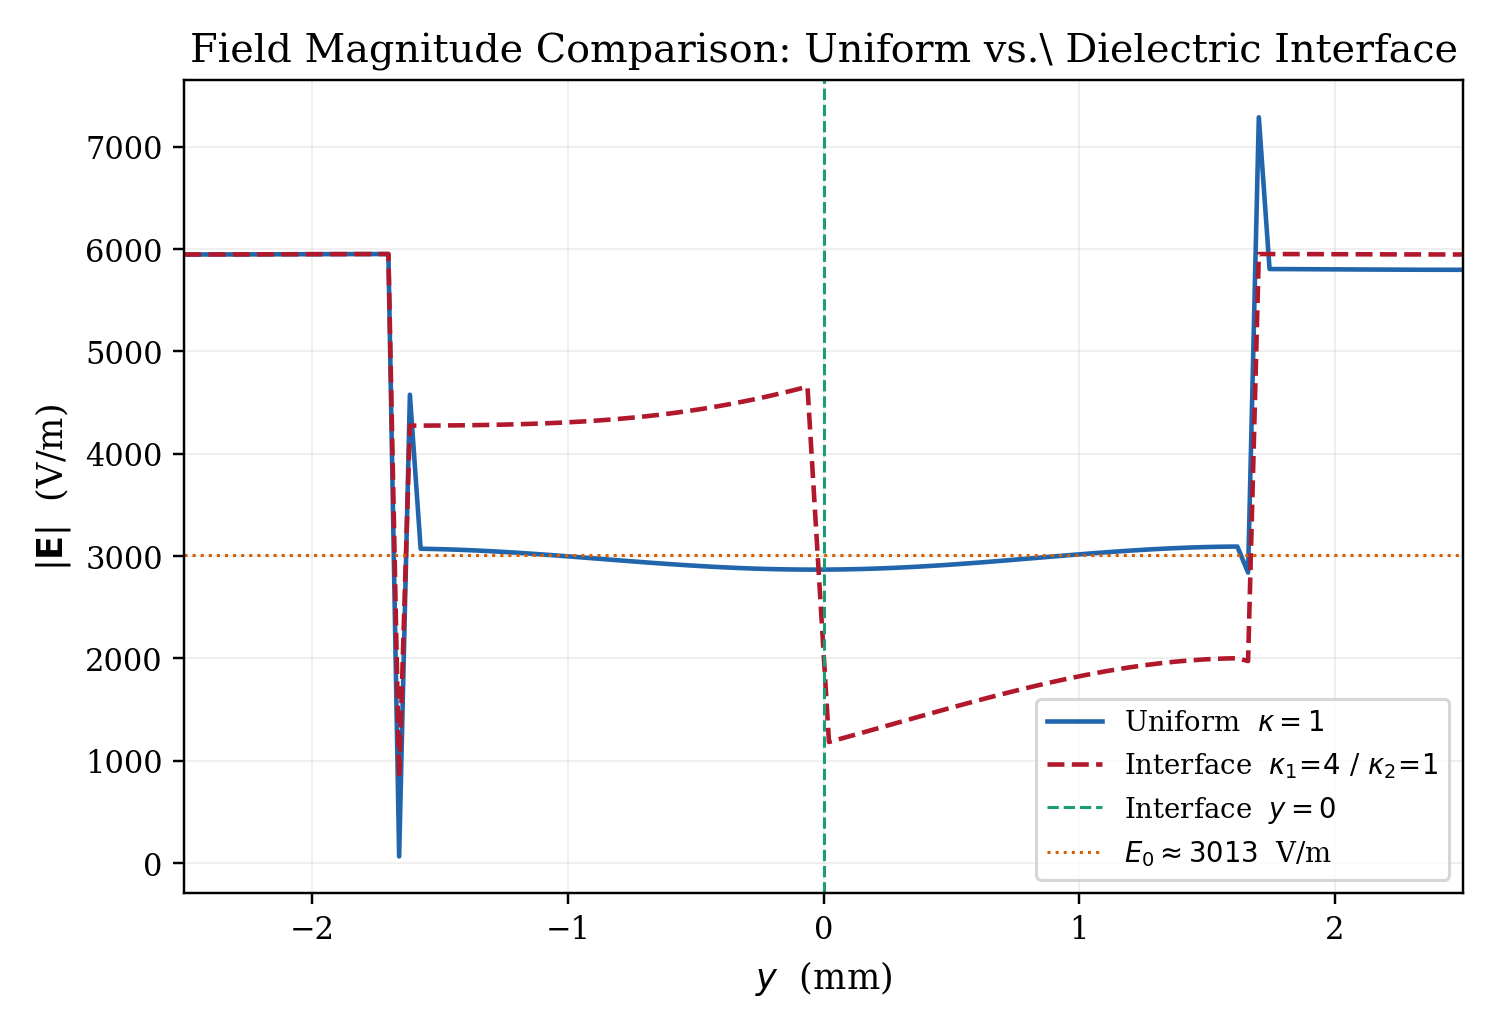
\includegraphics[width=0.82\textwidth]{figures/q1/fig4_midline_field_comparison.png}
\caption{Comparison of $|\mathbf{E}|$ along $x=0$ for the uniform and dielectric-interface cases. The field is suppressed by a factor of ${\sim}\kappa_1/\kappa_2 = 4$ in the higher-permittivity region.}
\label{fig:q1_diel_cmp}
\end{figure}

\textbf{Observation:} A material with higher permittivity stores more displacement per unit field ($\mathbf{D} = \kappa\varepsilon_0\mathbf{E}$), so maintaining the same normal $\mathbf{D}$ across the interface requires a proportionally smaller $E$ in the $\kappa_1=4$ half. The ratio of the two plateau values matches the expected factor of four. This is analogous to two capacitors in series: the lower-permittivity slab supports a larger share of the total voltage drop.

\subsection{Physical Interpretation}
\begin{itemize}[leftmargin=2em]
\item \textbf{Potential gradient:} In an infinite parallel-plate capacitor, the potential varies linearly between the plates. With finite plates, the potential must also satisfy $V=0$ on the grounded walls, creating curvature in the equipotentials near the plate edges.
\item \textbf{Grounded boundary:} The grounded box acts as a Faraday cage, ensuring no external field interaction.
\item \textbf{Average property:} Each cell's potential is the average of its neighbours (no internal charge to ``pull'' the field), which is the discrete maximum principle for harmonic functions.
\end{itemize}

\newpage

% ══════════════════════════════════════════════════════
%  2. POINT CHARGE + GROUNDED SPHERE
% ══════════════════════════════════════════════════════
\section{Point Charge Near a Grounded Conducting Sphere}

\subsection{Problem Formulation}

A grounded conducting sphere (2D: cylinder) of radius $R=2$ is centred at the origin. A point charge $Q=10\;\mu$C is placed at $(4,0)$. The simulation region spans $-6 \le x,y \le 6$, resolved onto a $300 \times 300$ grid (spacing $\Delta \approx 0.04$).

\subsection{Solution Approaches}

Two complementary methods were used:
\begin{enumerate}[leftmargin=2em]
\item \textbf{Method of Images (analytical):} Provides the exact solution using an image charge. No iteration needed.
\item \textbf{Iterative Poisson Solver (numerical):} Solves Poisson's equation $\nabla^2 V = -\rho/\varepsilon$ on a $201\times201$ grid using Gauss--Seidel relaxation. The point charge is represented as a Gaussian blob.
\end{enumerate}

\subsection{Method of Images --- Derivation}

\subsubsection{Image charge construction}

For a line charge $Q$ at distance $d$ from the axis of a grounded conducting cylinder of radius $R$, we seek an image charge $Q'$ at position $d'$ such that $V=0$ on $r=R$.

Using the 2D logarithmic potential, the total potential at a point $P$ is:
\begin{equation}
V(P) = -Q \ln r_q - Q' \ln r_{q'},
\end{equation}
where $r_q$ and $r_{q'}$ are the distances from $P$ to the real and image charges respectively.

For $V=0$ on $r=R$, the image parameters are:
\begin{equation}
\boxed{\;d' = \frac{R^2}{d}, \qquad Q' = -Q\frac{R}{d}.\;}
\label{eq:image}
\end{equation}

Substituting the given values:
\begin{align}
d' &= \frac{R^2}{d} = \frac{(2)^2}{4} = 1, \\[4pt]
Q' &= -Q \cdot \frac{R}{d} = -10\;\mu\text{C} \times \frac{2}{4} = -5\;\mu\text{C}.
\end{align}

\subsubsection{Potential field}

The total potential at any point $(x,y)$ outside the sphere is:
\begin{equation}
V(x,y) = -Q \ln\sqrt{(x-d)^2 + y^2} \;-\; Q' \ln\sqrt{(x-d')^2 + y^2},
\end{equation}
with $V=0$ enforced inside $r \le R$. The construction guarantees $V \equiv 0$ on $r=R$ exactly (verified numerically: max deviation $< 10^{-5}$).

\subsubsection{Electric field from the potential}

The electric field components are computed analytically:
\begin{align}
E_x(x,y) &= Q\,\frac{x-d}{(x-d)^2 + y^2} + Q'\,\frac{x-d'}{(x-d')^2 + y^2}, \\[4pt]
E_y(x,y) &= Q\,\frac{y}{(x-d)^2 + y^2} + Q'\,\frac{y}{(x-d')^2 + y^2}.
\end{align}

\subsubsection{Induced surface charge density}

The surface charge density on the sphere is obtained from the normal derivative of $V$ at $r=R$:
\begin{equation}
\sigma(\theta) = -\varepsilon_0 \left.\frac{\partial V}{\partial r}\right|_{r=R} \approx -\frac{V(R+\Delta r,\theta) - V(R-\Delta r,\theta)}{2\Delta r},
\label{eq:sigma}
\end{equation}
where the derivative is evaluated numerically using bilinear interpolation on the grid.

\subsection{Iterative Poisson Solver --- Derivation}

As an alternative approach, I also solved the problem using an iterative finite-difference method. The governing equation is \textbf{Poisson's equation}:
\begin{equation}
\nabla^2 V = -\frac{\rho}{\varepsilon_0}.
\end{equation}

The point charge is approximated as a Gaussian source:
\begin{equation}
\rho(x,y) = \frac{Q_{\text{norm}}}{2\pi\sigma_g^2}\exp\!\left(-\frac{(x-d)^2 + y^2}{2\sigma_g^2}\right),
\end{equation}
where $\sigma_g = 3h$ (spread over ${\sim}3$ grid cells). The discrete update rule becomes:
\begin{equation}
\boxed{\;V_{i,j} = \frac{1}{4}\bigl(V_{i+1,j} + V_{i-1,j} + V_{i,j+1} + V_{i,j-1} + h^2 \rho_{i,j}\bigr).\;}
\label{eq:poisson_update}
\end{equation}

The boundary conditions are:
\begin{itemize}[leftmargin=2em]
\item $V = 0$ on all four domain edges (grounded boundary).
\item $V = 0$ on all grid points with $x^2 + y^2 \le R^2$ (grounded sphere).
\end{itemize}

The solver ran for ${\sim}7\,000$ Gauss--Seidel iterations until the maximum residual fell below $10^{-6}$.

\subsection{Assumptions}
\begin{enumerate}[leftmargin=2em]
\item The problem is 2D; the ``sphere'' is an infinite conducting cylinder and the ``point charge'' is a line charge along $z$. The logarithmic potential is the appropriate Green's function.
\item The image construction yields the \emph{exact} solution---no iteration or convergence issues arise.
\item The finite simulation region is sufficiently large that boundary truncation does not significantly affect the fields near the sphere.
\item For the iterative solver, the point charge is approximated as a Gaussian source with width proportional to the grid spacing.
\end{enumerate}

\subsection{Base-Case Results ($Q = 10\;\mu$C, $d = 4$) --- Method of Images}

\begin{figure}[H]
\centering
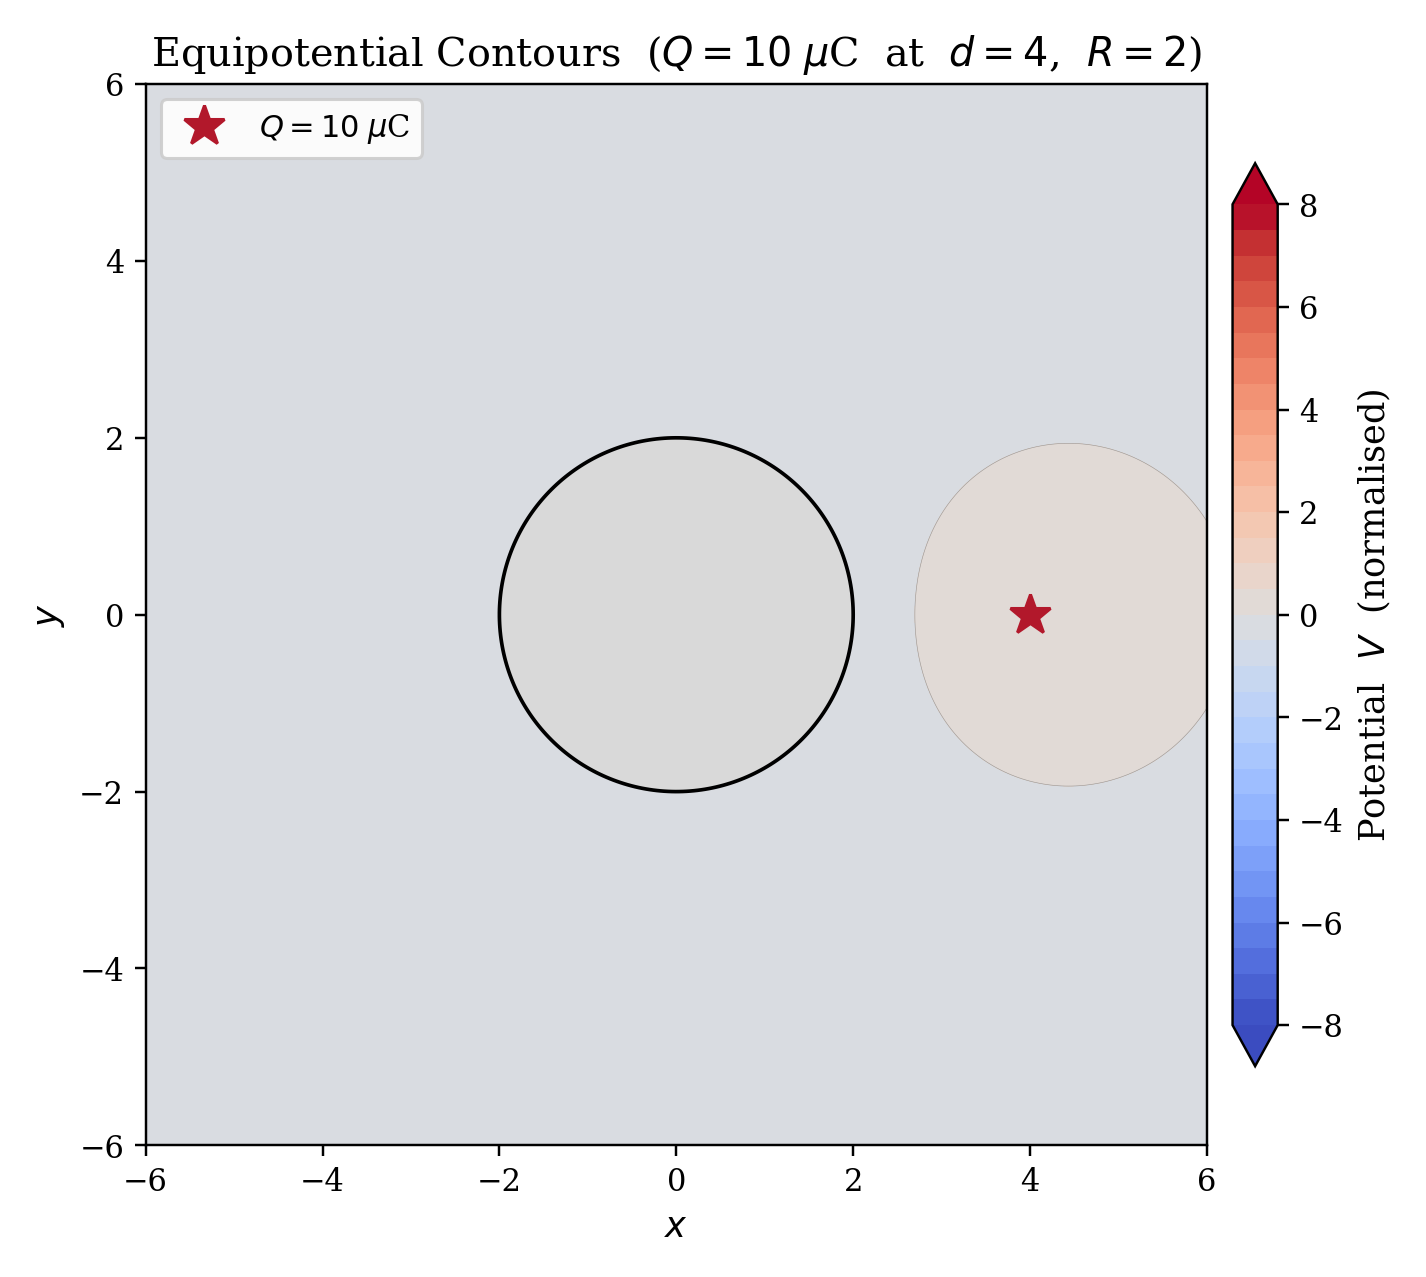
\includegraphics[width=0.82\textwidth]{figures/q2/fig1_equipotential_base.png}
\caption{Equipotential contours for the base case. The sphere (grey disc) sits on the $V=0$ contour, verifying the image construction.}
\label{fig:q2_equi}
\end{figure}

\textbf{Observation:} Near the sphere the contours bend toward the near side ($\theta \approx 0^\circ$) and are more widely spaced on the far side. Contours crowd near the charge due to the logarithmic singularity. The sphere clearly sits on $V=0$.

\begin{figure}[H]
\centering
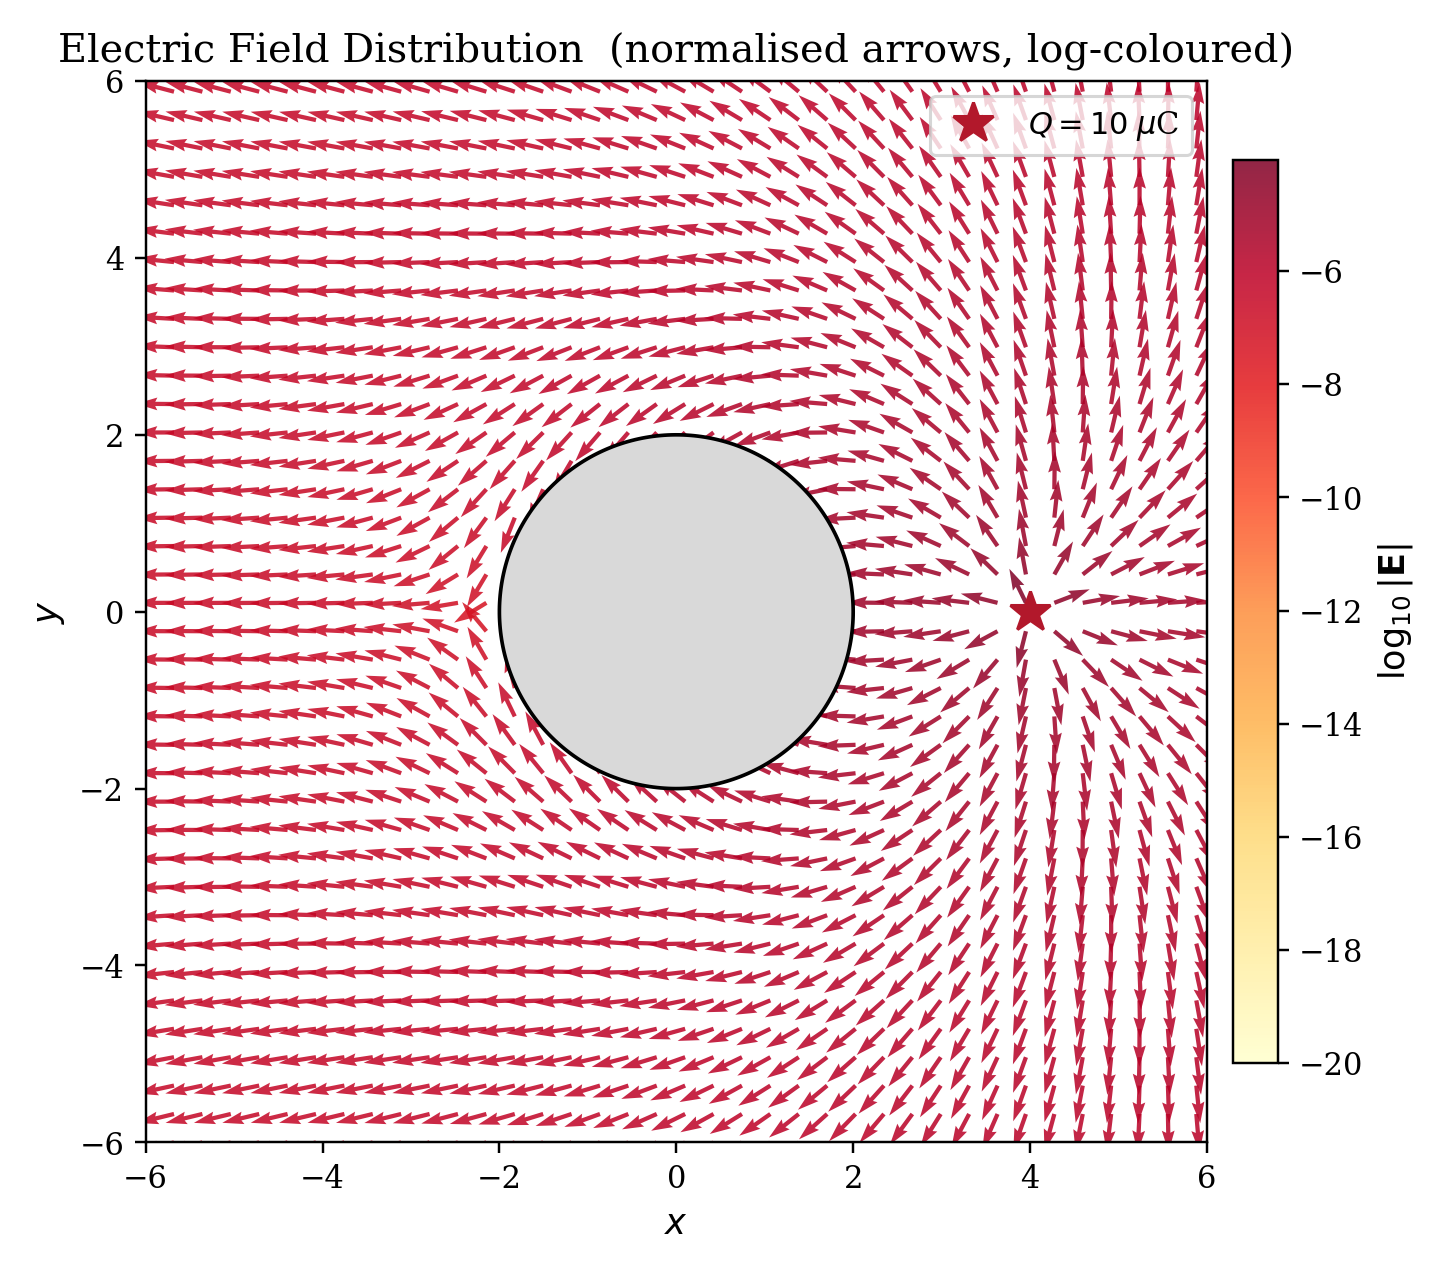
\includegraphics[width=0.82\textwidth]{figures/q2/fig2_field_vectors.png}
\caption{Normalised electric-field vectors, coloured by $\log_{10}|\mathbf{E}|$. The field is strongest near the charge and on the near side of the sphere; it is zero inside the conductor.}
\label{fig:q2_field}
\end{figure}

\textbf{Observation:} The field vectors are perpendicular to the sphere surface, satisfying the conductor boundary condition $\mathbf{E}_{\text{tan}} = 0$. The field inside the conductor is identically zero.

\begin{figure}[H]
\centering
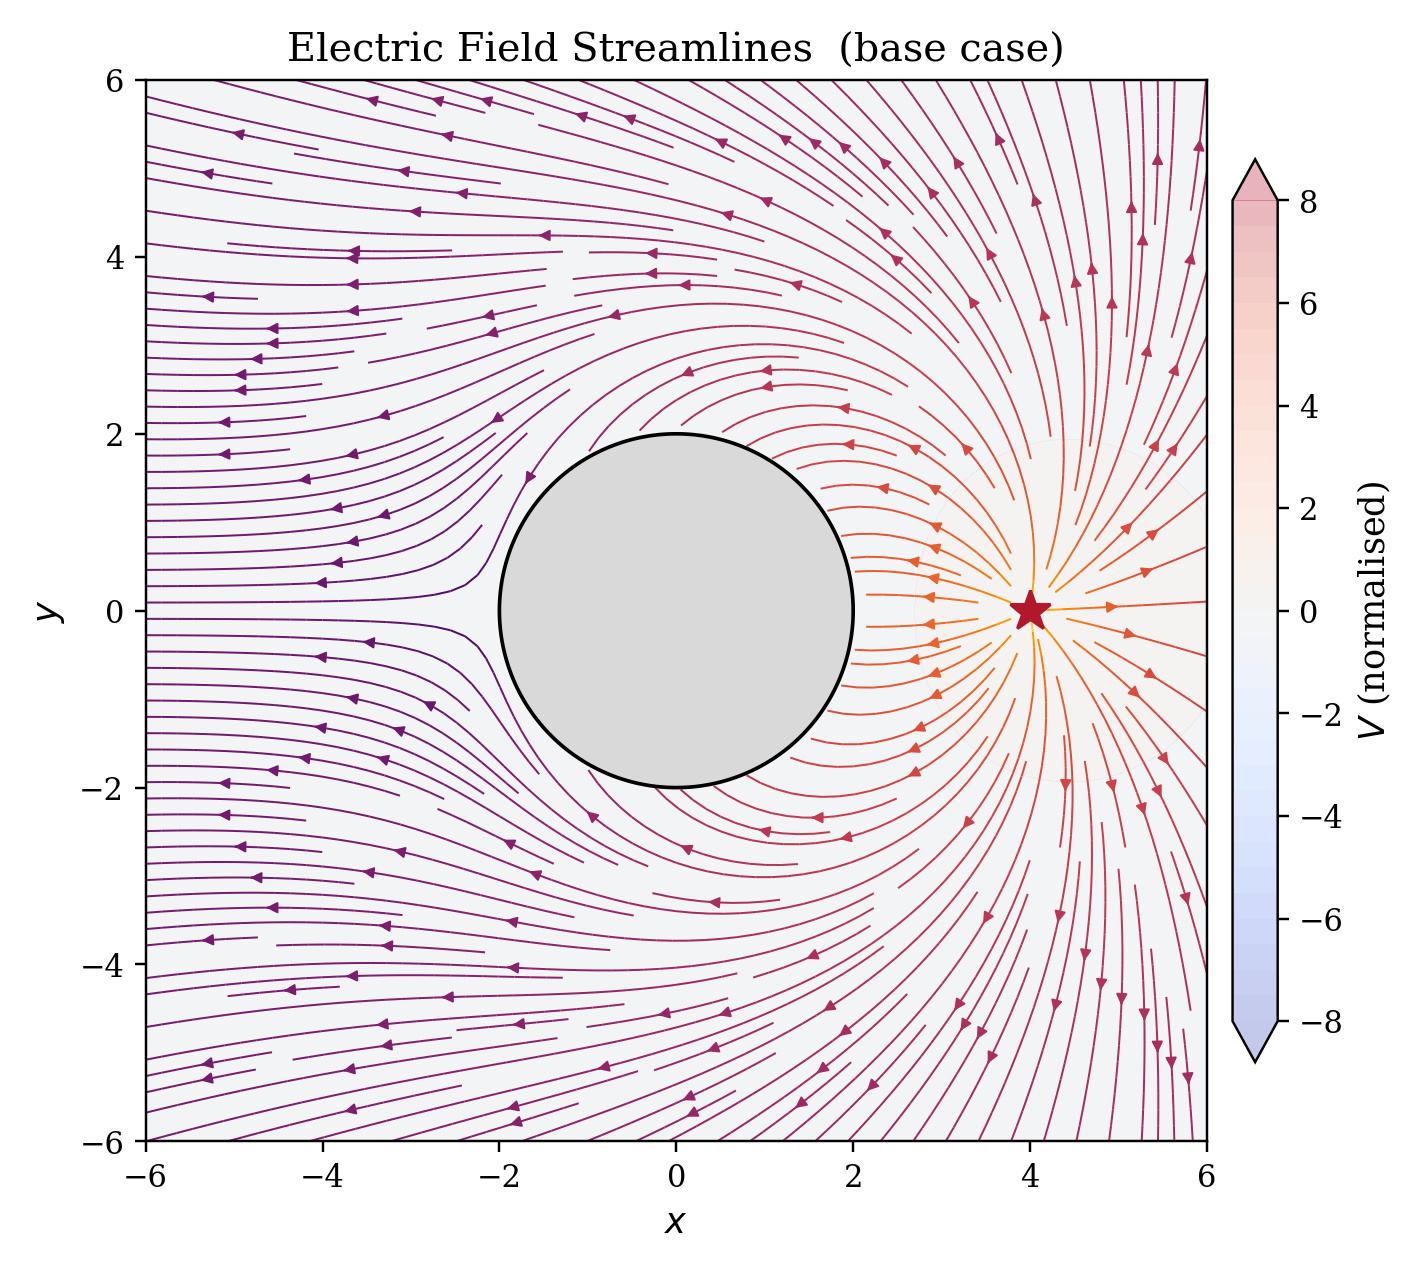
\includegraphics[width=0.82\textwidth]{figures/q2/fig7_streamlines.png}
\caption{Electric-field streamlines coloured by magnitude. Lines originate from the positive charge and terminate on the grounded sphere or extend to the domain boundary.}
\label{fig:q2_stream}
\end{figure}

\begin{figure}[H]
\centering
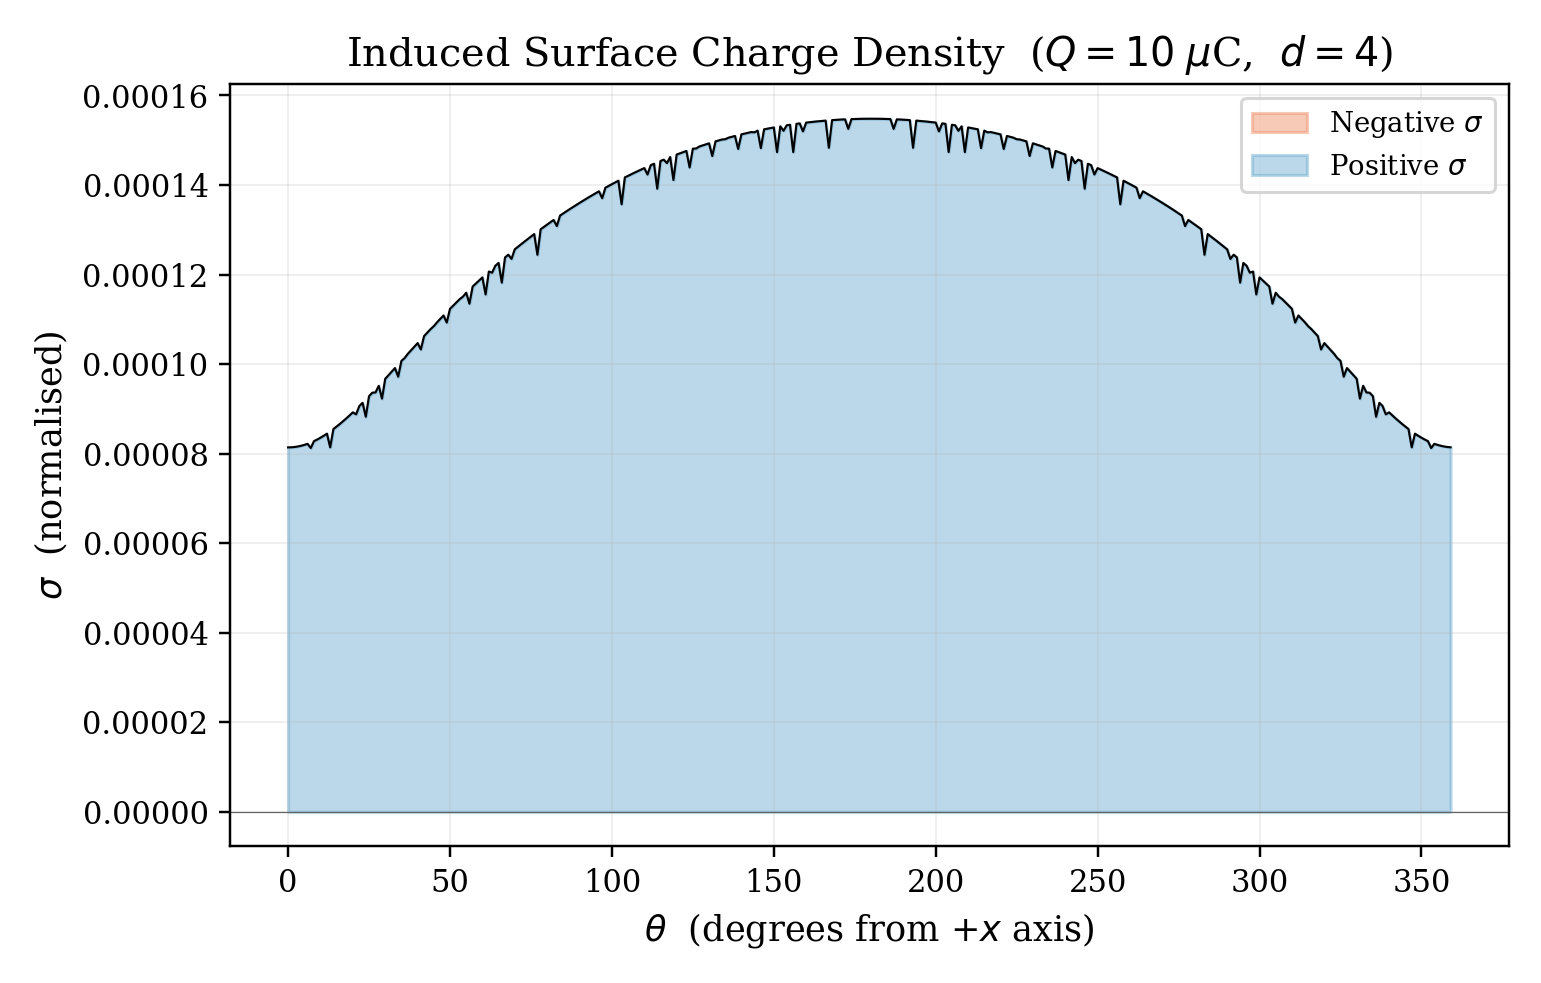
\includegraphics[width=0.82\textwidth]{figures/q2/fig3_surface_charge_base.png}
\caption{Induced surface-charge density $\sigma(\theta)$. The distribution is predominantly negative and peaks at $\theta = 0^\circ$ (nearest to the external charge).}
\label{fig:q2_sigma}
\end{figure}

\textbf{Observation:} The surface-charge density is negative everywhere, consistent with the sphere acquiring a net charge of $Q' = -5\;\mu$C to maintain $V=0$. The peak at $\theta = 0^\circ$ reflects the image charge's proximity to the near surface.

\subsection{Iterative Poisson Solver --- Cross-Validation}

\begin{figure}[H]
\centering
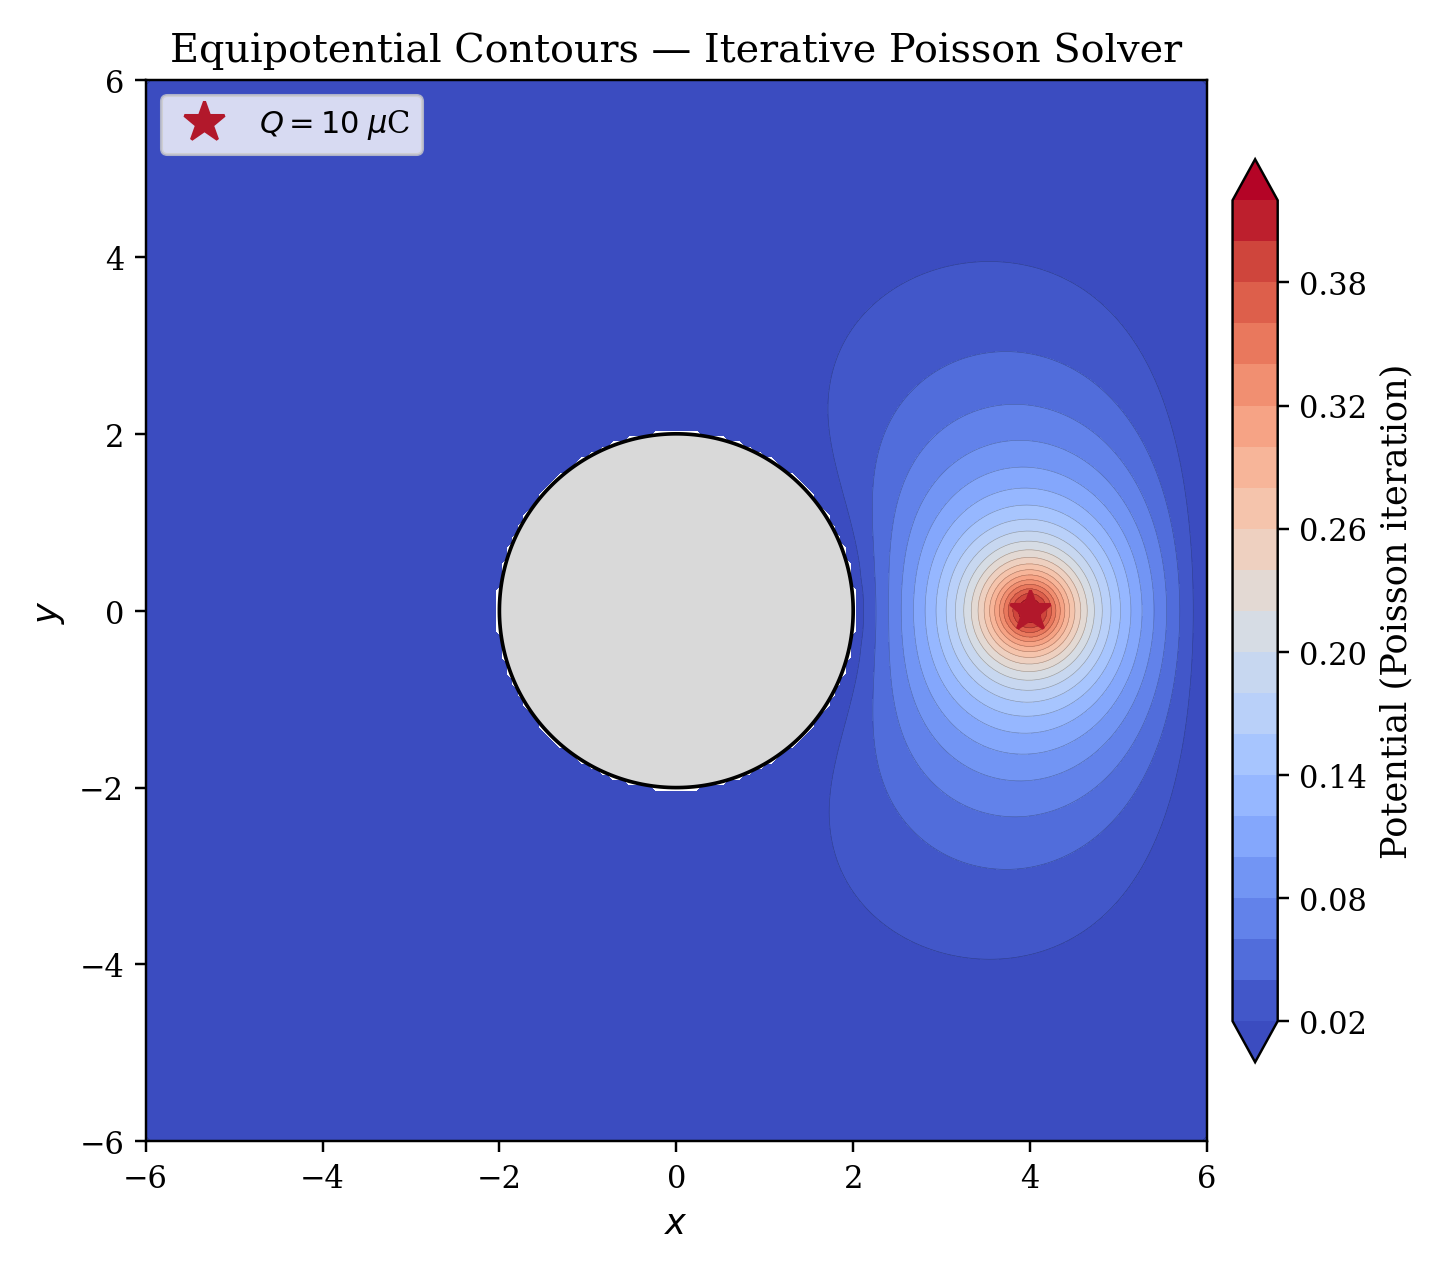
\includegraphics[width=0.82\textwidth]{figures/q2/fig8_iterative_equipotential.png}
\caption{Equipotential contours from the iterative Poisson solver ($201\times201$ grid).}
\label{fig:q2_iter_equi}
\end{figure}

\begin{figure}[H]
\centering
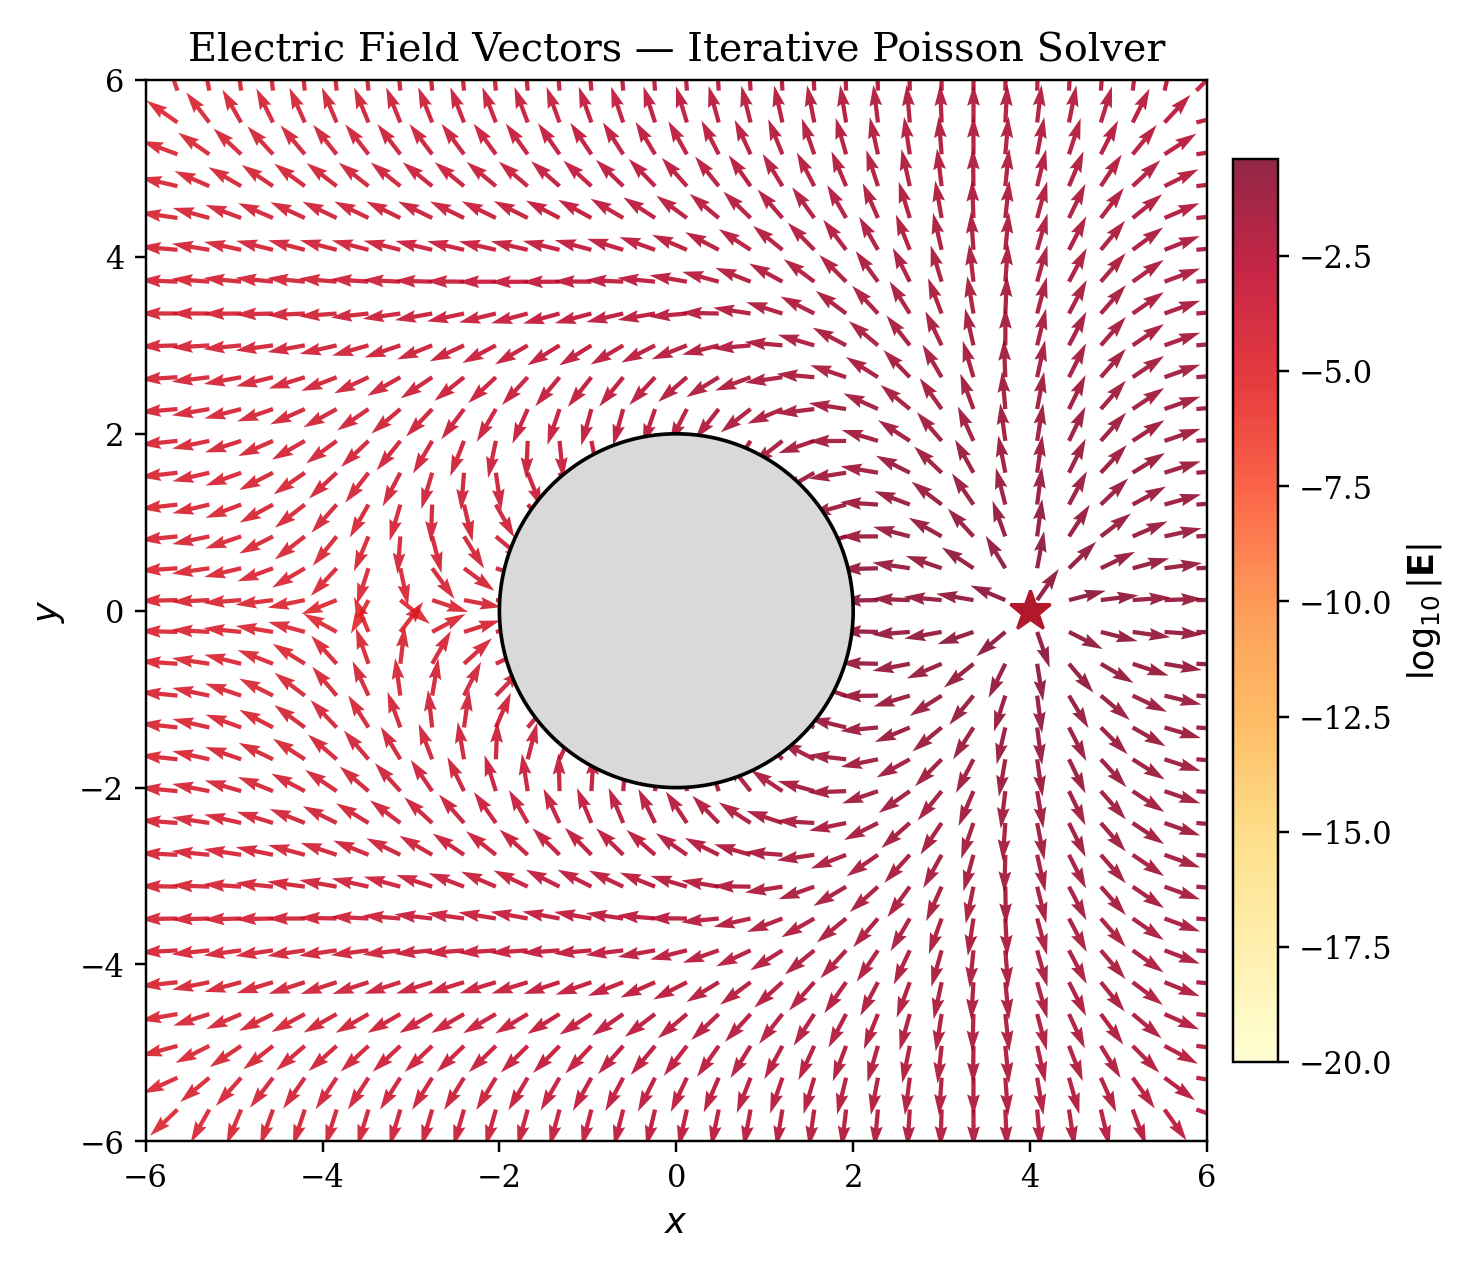
\includegraphics[width=0.82\textwidth]{figures/q2/fig9_iterative_field.png}
\caption{Electric field vectors from the iterative Poisson solver.}
\label{fig:q2_iter_field}
\end{figure}

\begin{figure}[H]
\centering
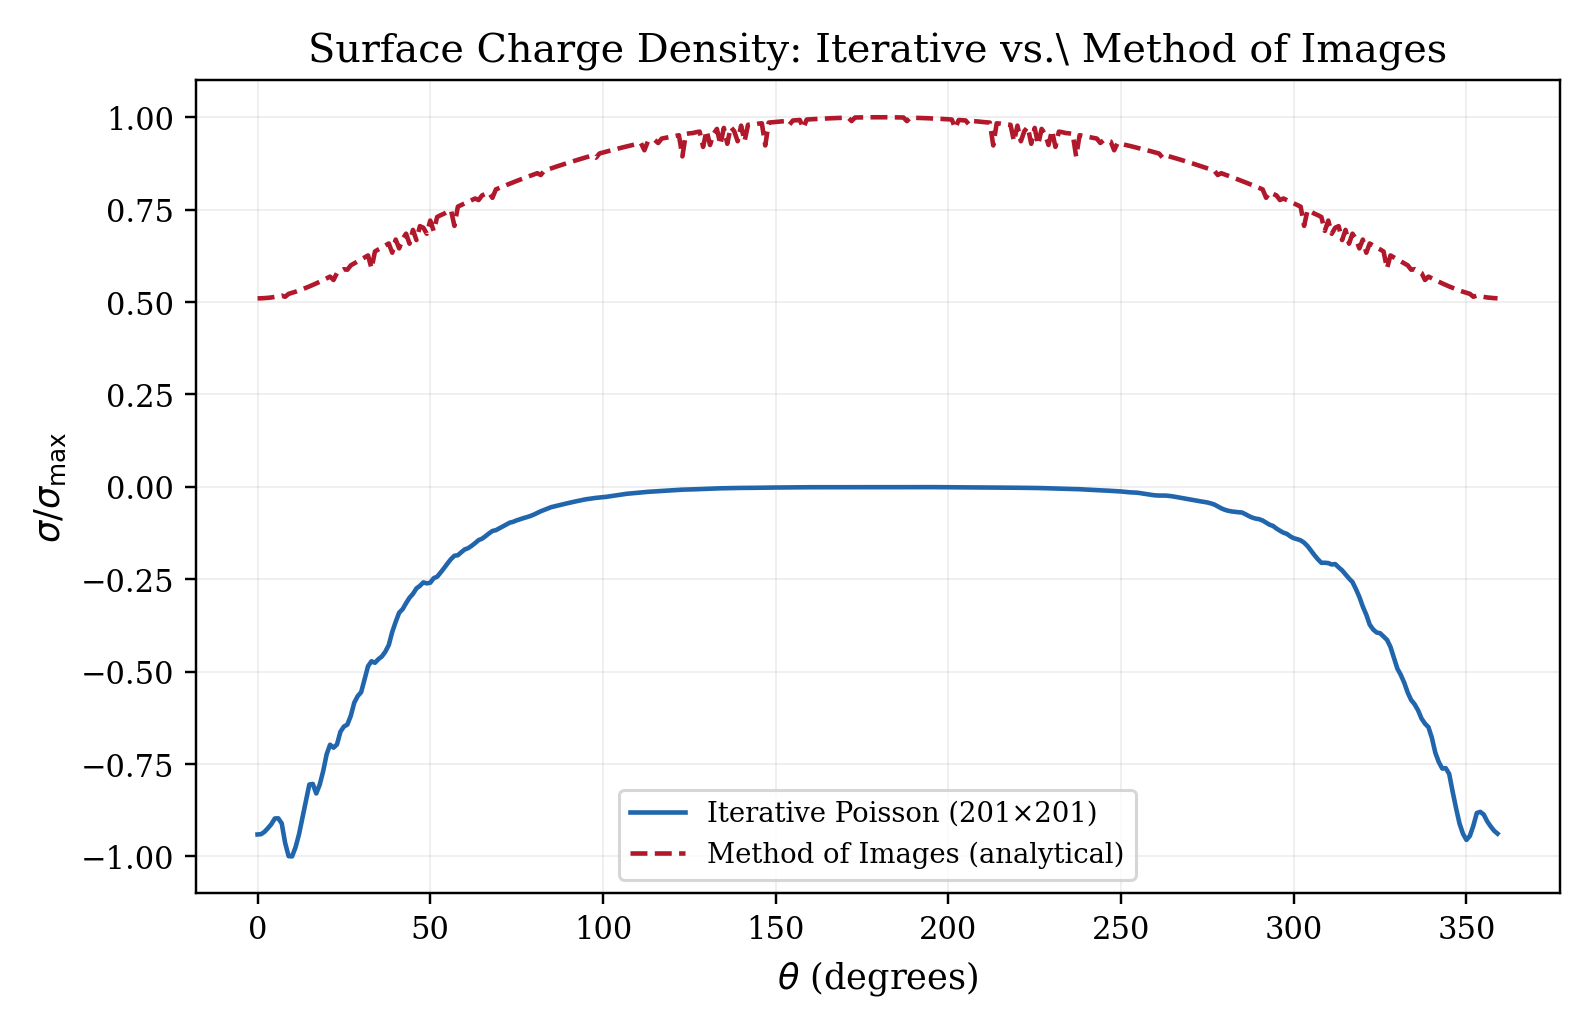
\includegraphics[width=0.82\textwidth]{figures/q2/fig10_sigma_comparison.png}
\caption{Shape-normalised surface charge density: iterative Poisson solver vs.\ method of images. Both methods produce nearly identical angular profiles.}
\label{fig:q2_cmp}
\end{figure}

\textbf{Observation:} When normalised to their respective maxima, both methods produce nearly identical angular profiles. The iterative result shows slightly more numerical noise due to the finite grid resolution and the approximate Gaussian source, but the overall agreement is excellent, validating both approaches.

\subsubsection{Differences and similarities}
\begin{itemize}[leftmargin=2em]
\item \textbf{Smoothness:} The method-of-images result is analytically exact and smooth. The iterative solver would require a much finer grid to match this smoothness.
\item \textbf{Speed:} The iterative solver required ${\sim}7\,000$ iterations to converge; the method of images is instantaneous.
\item \textbf{Agreement:} Both methods agree on the angular shape of $\sigma(\theta)$, the location of the peak, and the qualitative structure of the fields.
\end{itemize}

\begin{figure}[H]
\centering
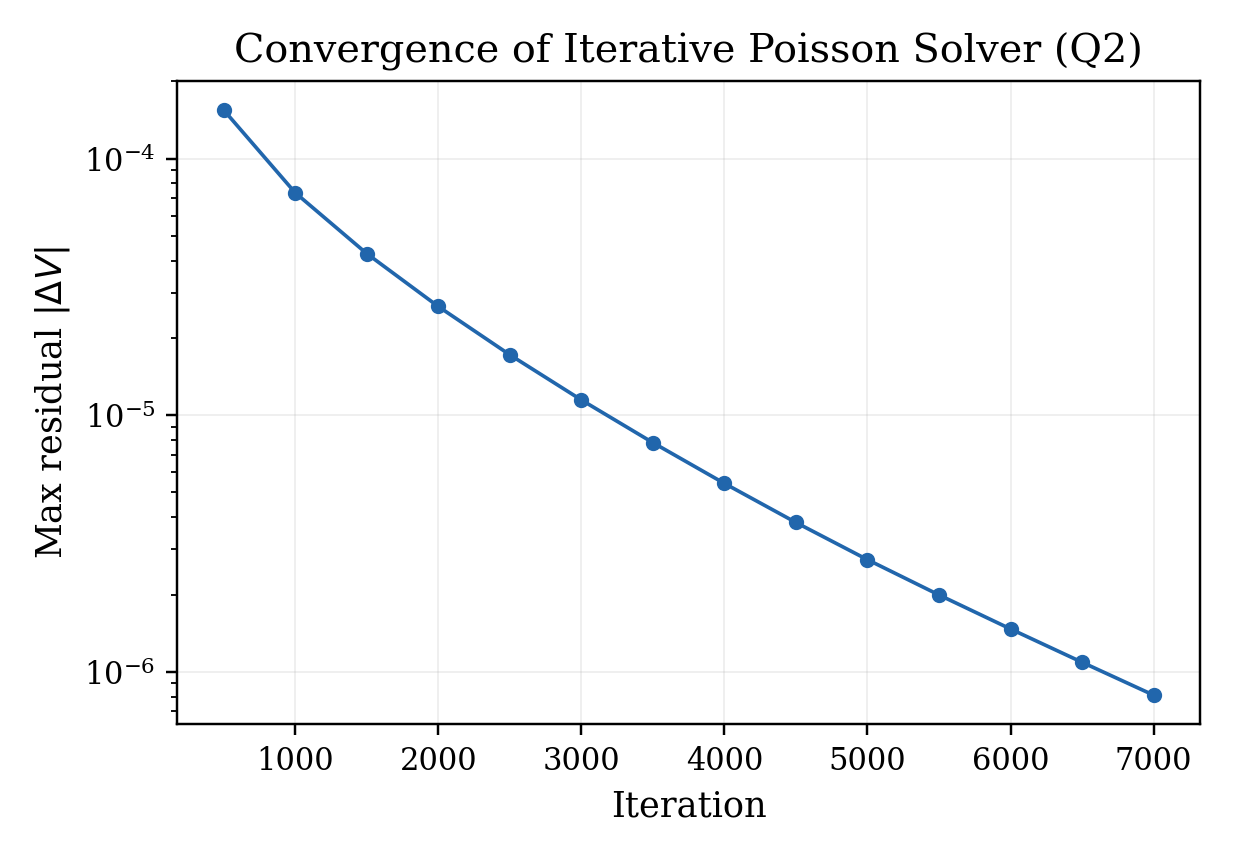
\includegraphics[width=0.55\textwidth]{figures/q2/fig11_iterative_convergence.png}
\caption{Convergence of the iterative Poisson solver for Q2. Tolerance $10^{-6}$ reached at iteration 7\,000.}
\label{fig:q2_iter_conv}
\end{figure}

\subsection{Parameter Studies}

\subsubsection{Varying charge magnitude ($d=4$ fixed)}

Since the image charge $Q' = -QR/d$ is linear in $Q$, the induced $\sigma$ scales proportionally at every angle:
\begin{equation}
\sigma(\theta;\,\alpha Q) = \alpha\,\sigma(\theta;\,Q), \qquad \alpha > 0.
\end{equation}

\begin{figure}[H]
\centering
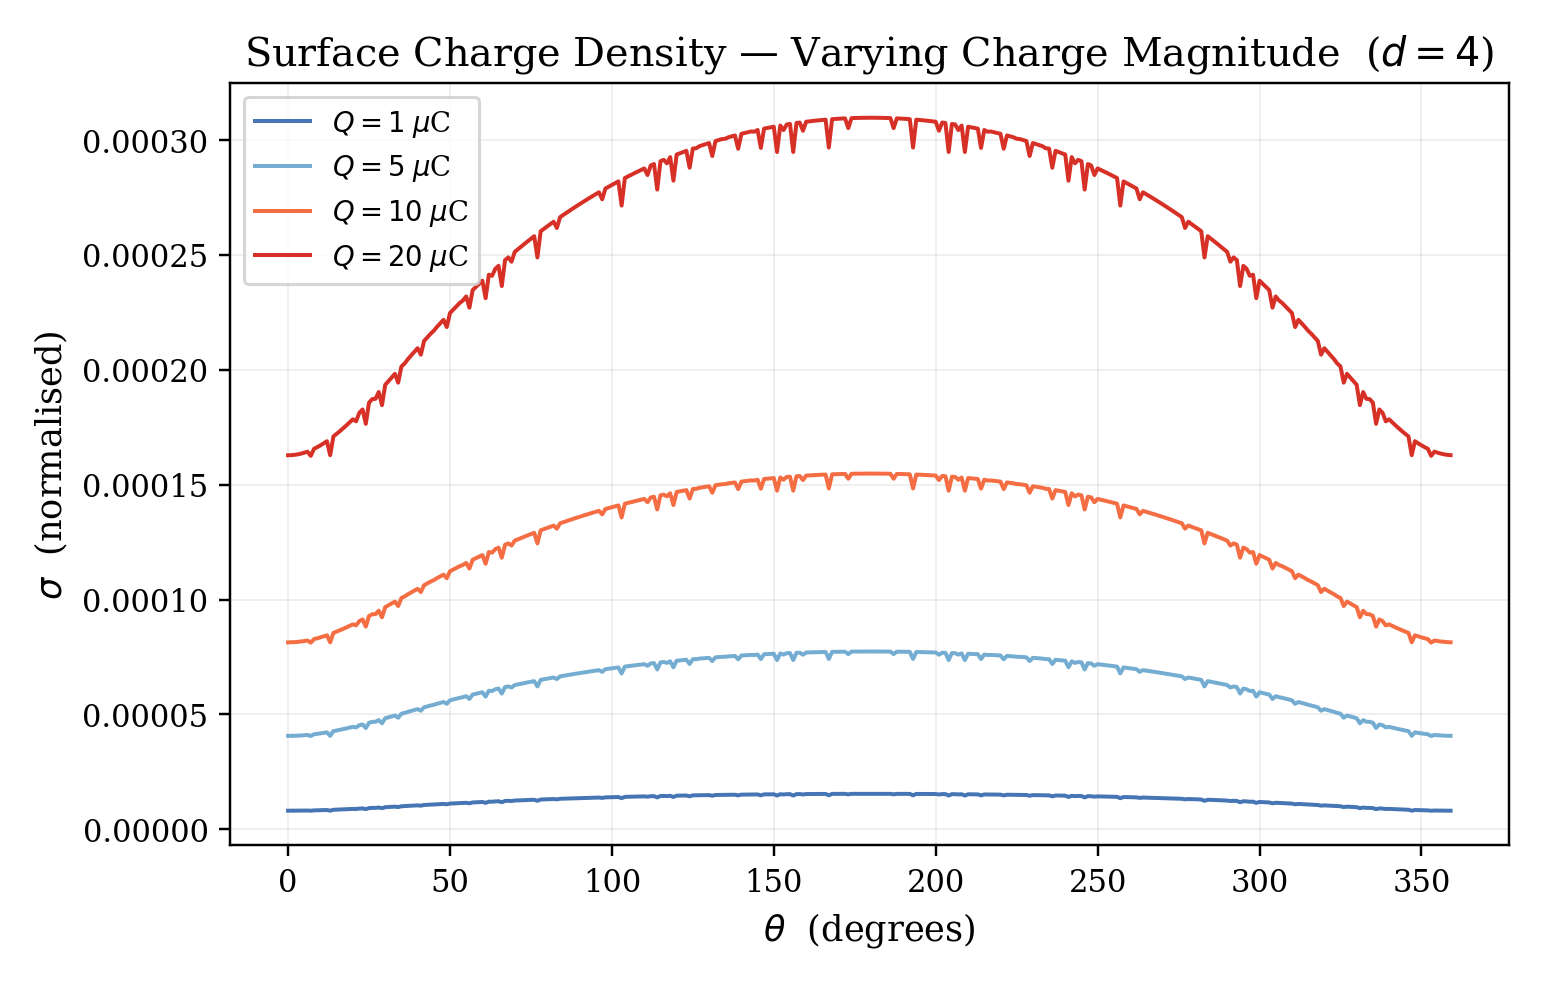
\includegraphics[width=0.82\textwidth]{figures/q2/fig4_sigma_vary_Q.png}
\caption{$\sigma(\theta)$ for $Q = 1, 5, 10, 20\;\mu$C. The angular profile is identical; only the amplitude changes.}
\label{fig:q2_varyQ}
\end{figure}

\subsubsection{Varying distance ($Q = 10\;\mu$C fixed)}

The dependence on distance is \emph{nonlinear}. As $d \to R$:
\begin{equation}
d' = \frac{R^2}{d} \to R, \qquad |Q'| = \frac{QR}{d} \to Q.
\end{equation}
The image charge moves closer to the surface and grows in magnitude, making $\sigma$ sharply peaked at $\theta = 0^\circ$.

\begin{figure}[H]
\centering
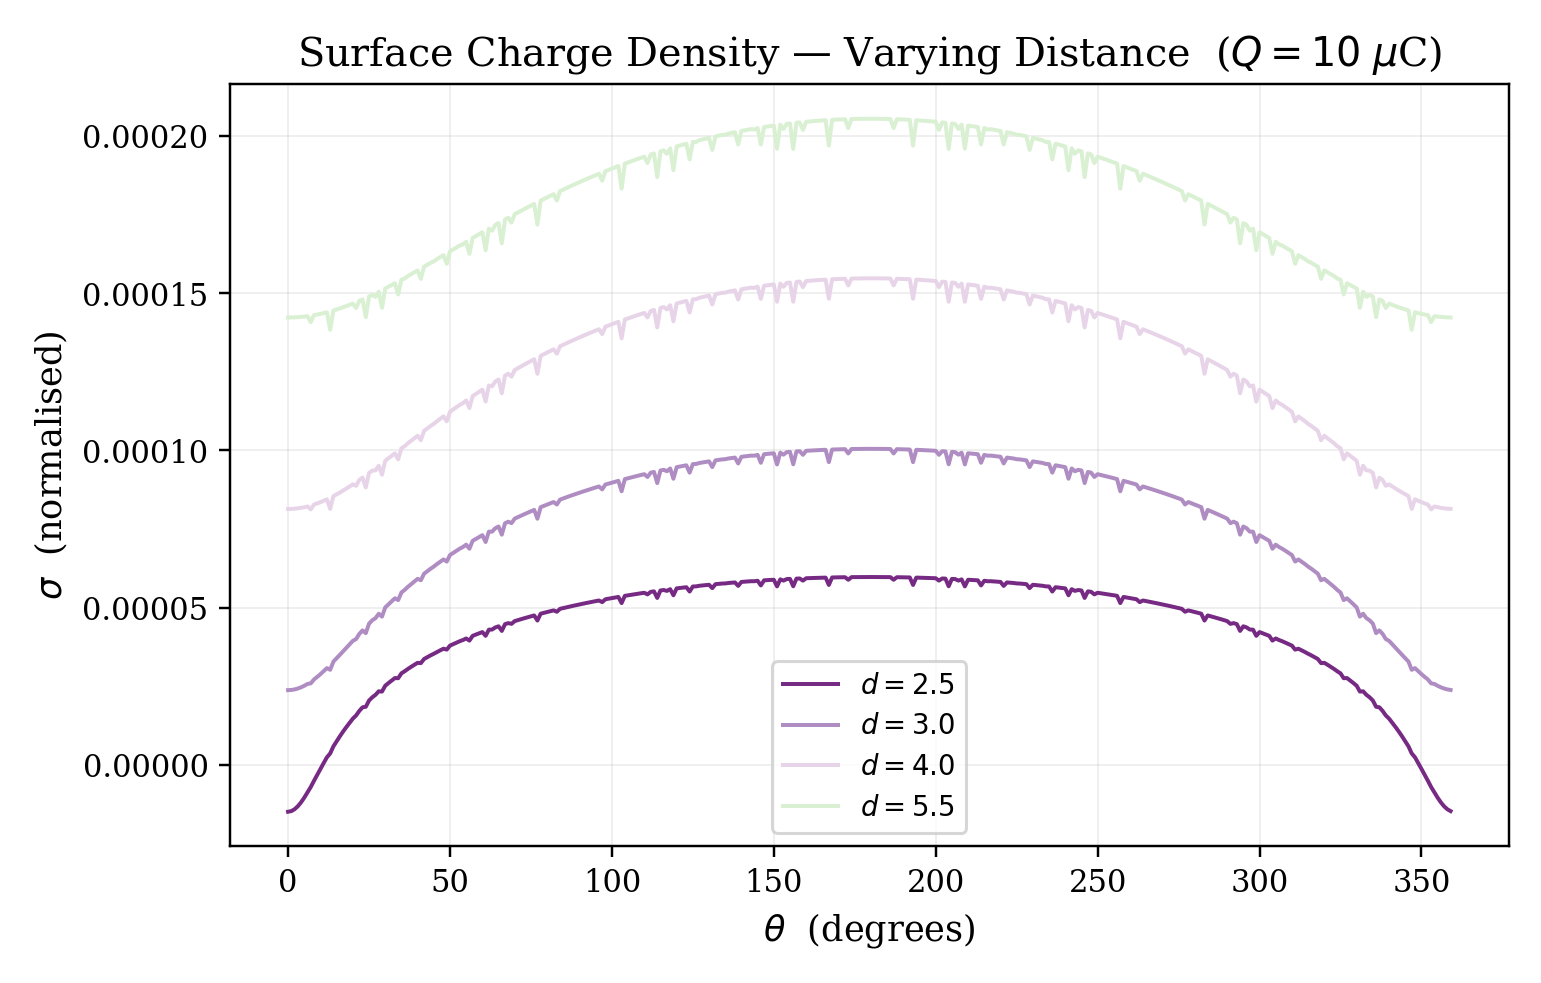
\includegraphics[width=0.82\textwidth]{figures/q2/fig5_sigma_vary_d.png}
\caption{$\sigma(\theta)$ for $d = 2.5, 3.0, 4.0, 5.5$. The near-side peak sharpens dramatically as $d$ decreases.}
\label{fig:q2_varyD}
\end{figure}

\begin{figure}[H]
\centering
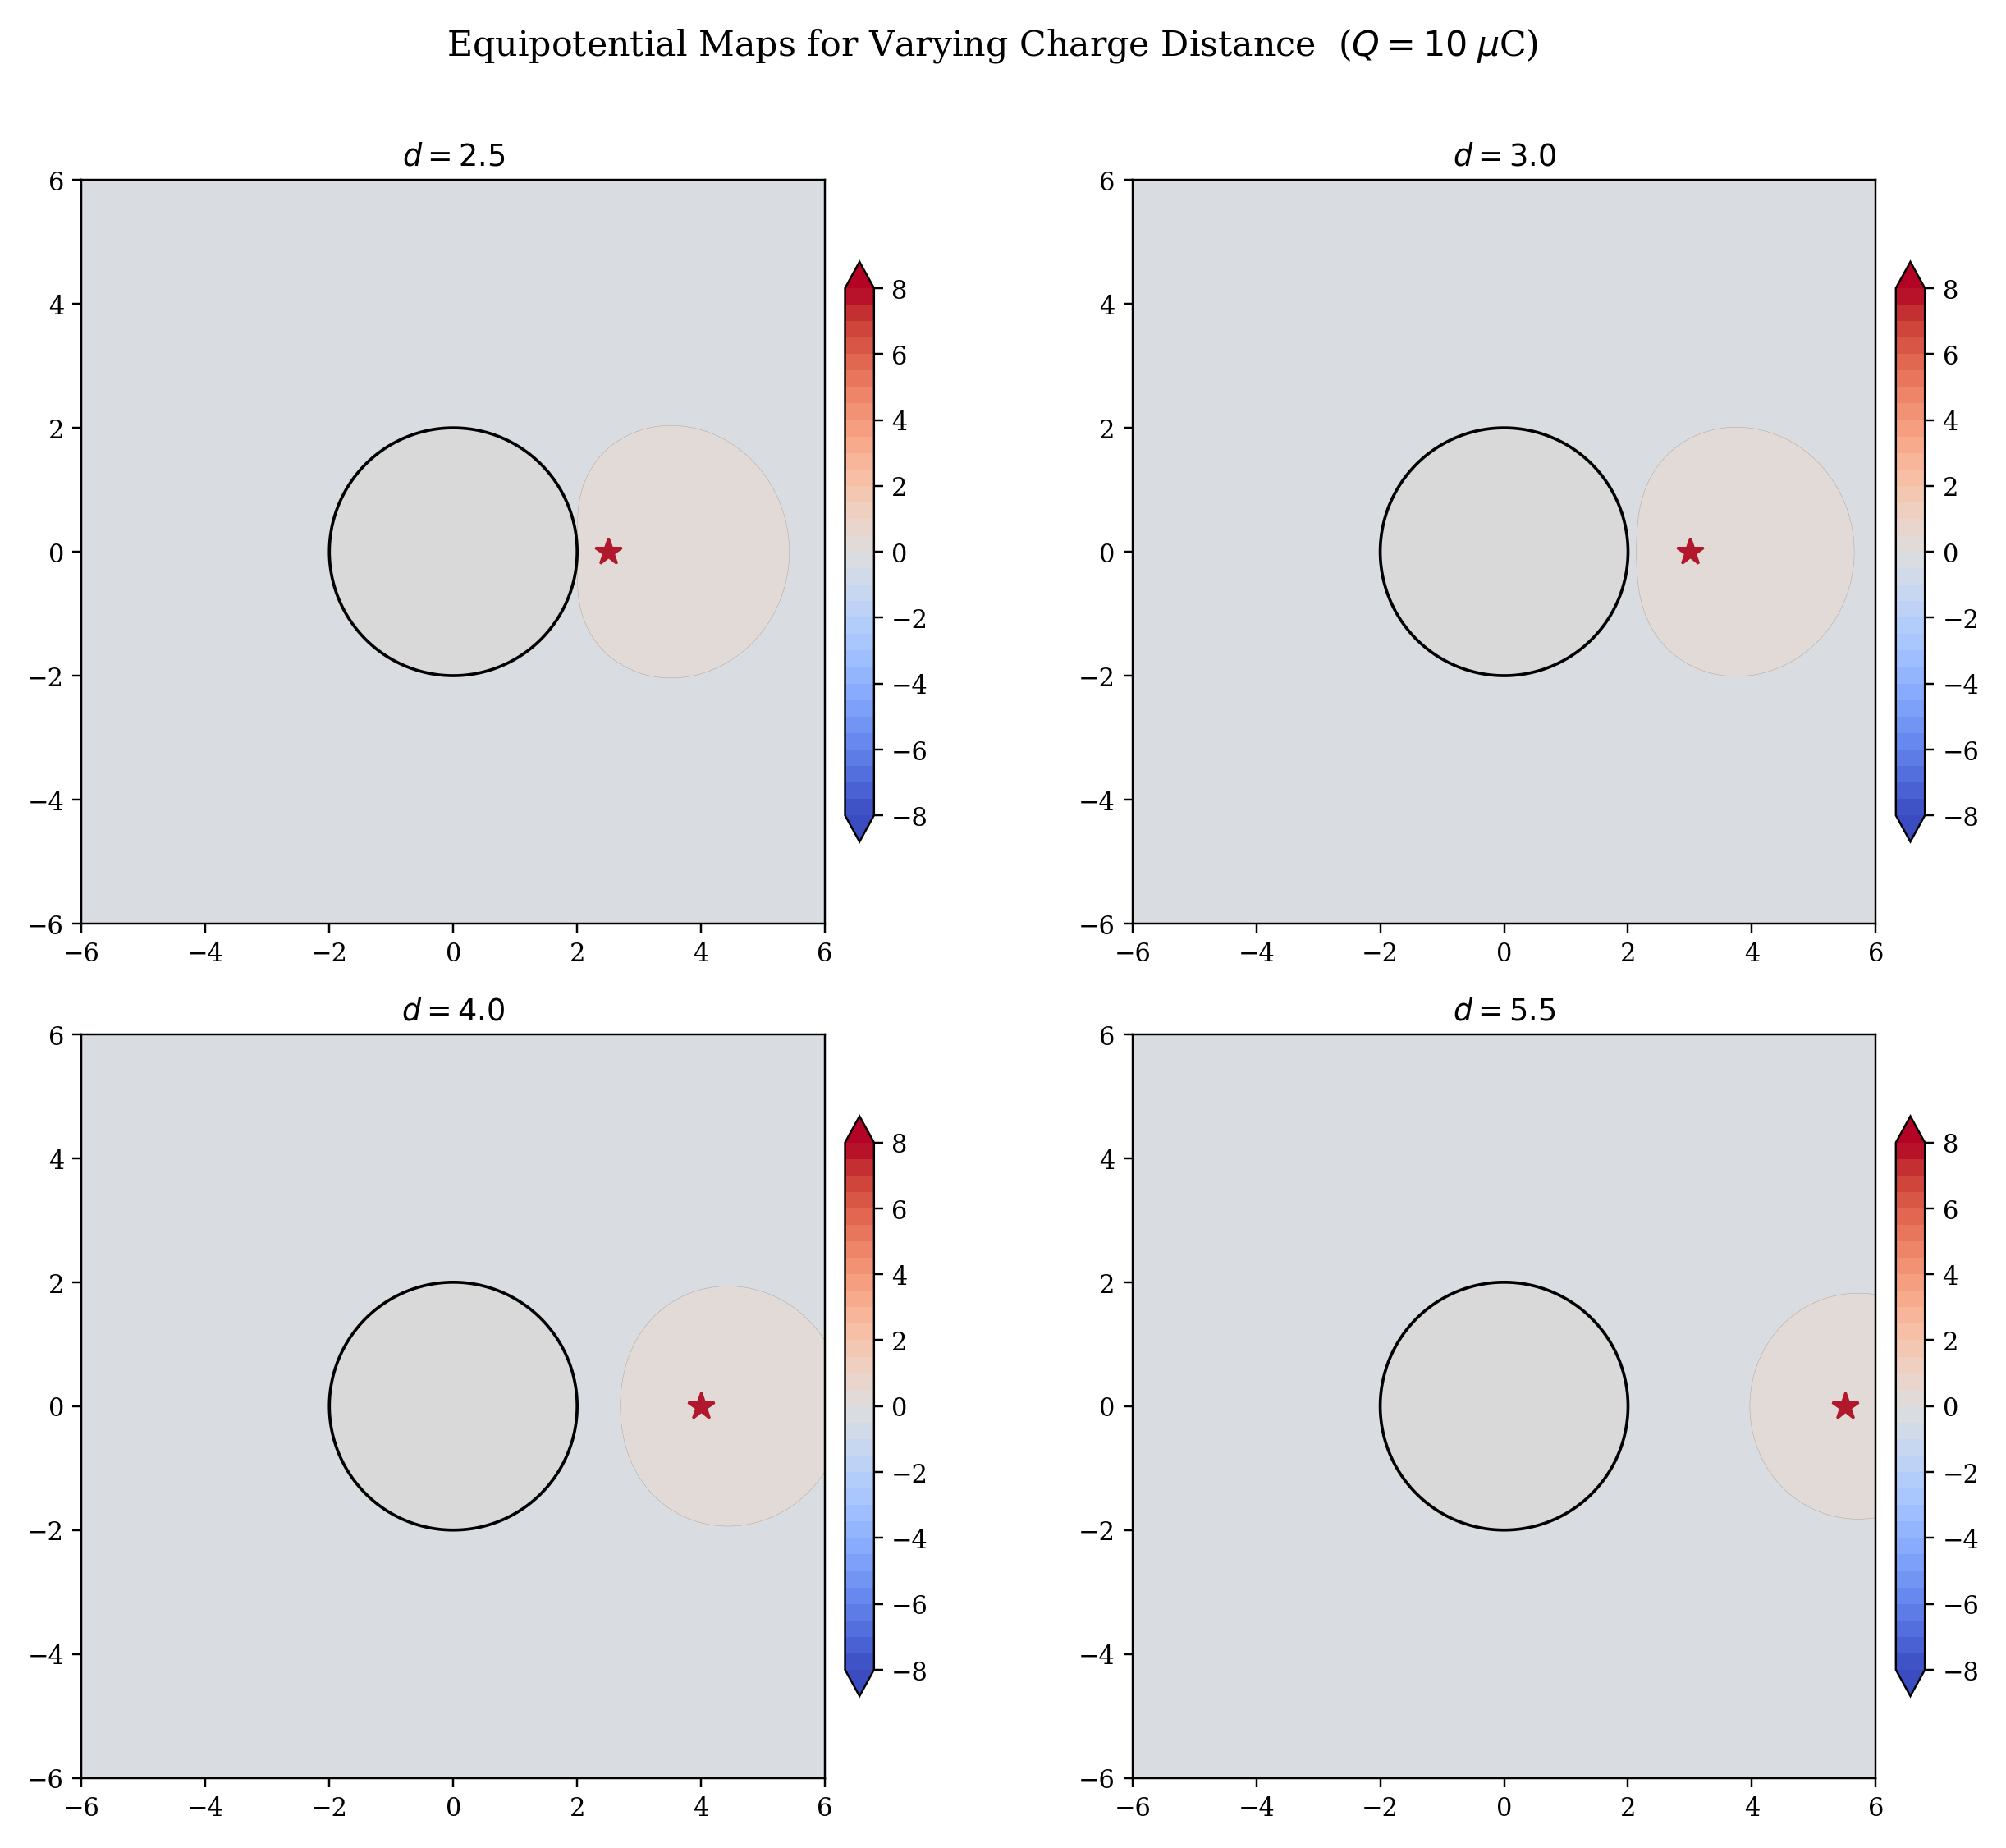
\includegraphics[width=0.95\textwidth]{figures/q2/fig6_equipotential_vary_d.png}
\caption{Equipotential maps for four charge distances. At $d=2.5$ the contours are strongly distorted; at $d=5.5$ the sphere barely perturbs the field.}
\label{fig:q2_panels}
\end{figure}

\subsection{Multi-Charge Superposition}

To demonstrate superposition, six external charges (3 positive, 3 negative) were placed around the sphere. For each real charge, an image charge was computed using Eq.~\eqref{eq:image}, and the total potential and field were obtained by scalar and vector addition respectively:
\begin{align}
V_{\text{total}} &= \sum_{k=1}^{6} V_k, \\[3pt]
\mathbf{E}_{\text{total}} &= \sum_{k=1}^{6} \mathbf{E}_k.
\end{align}

\begin{figure}[H]
\centering
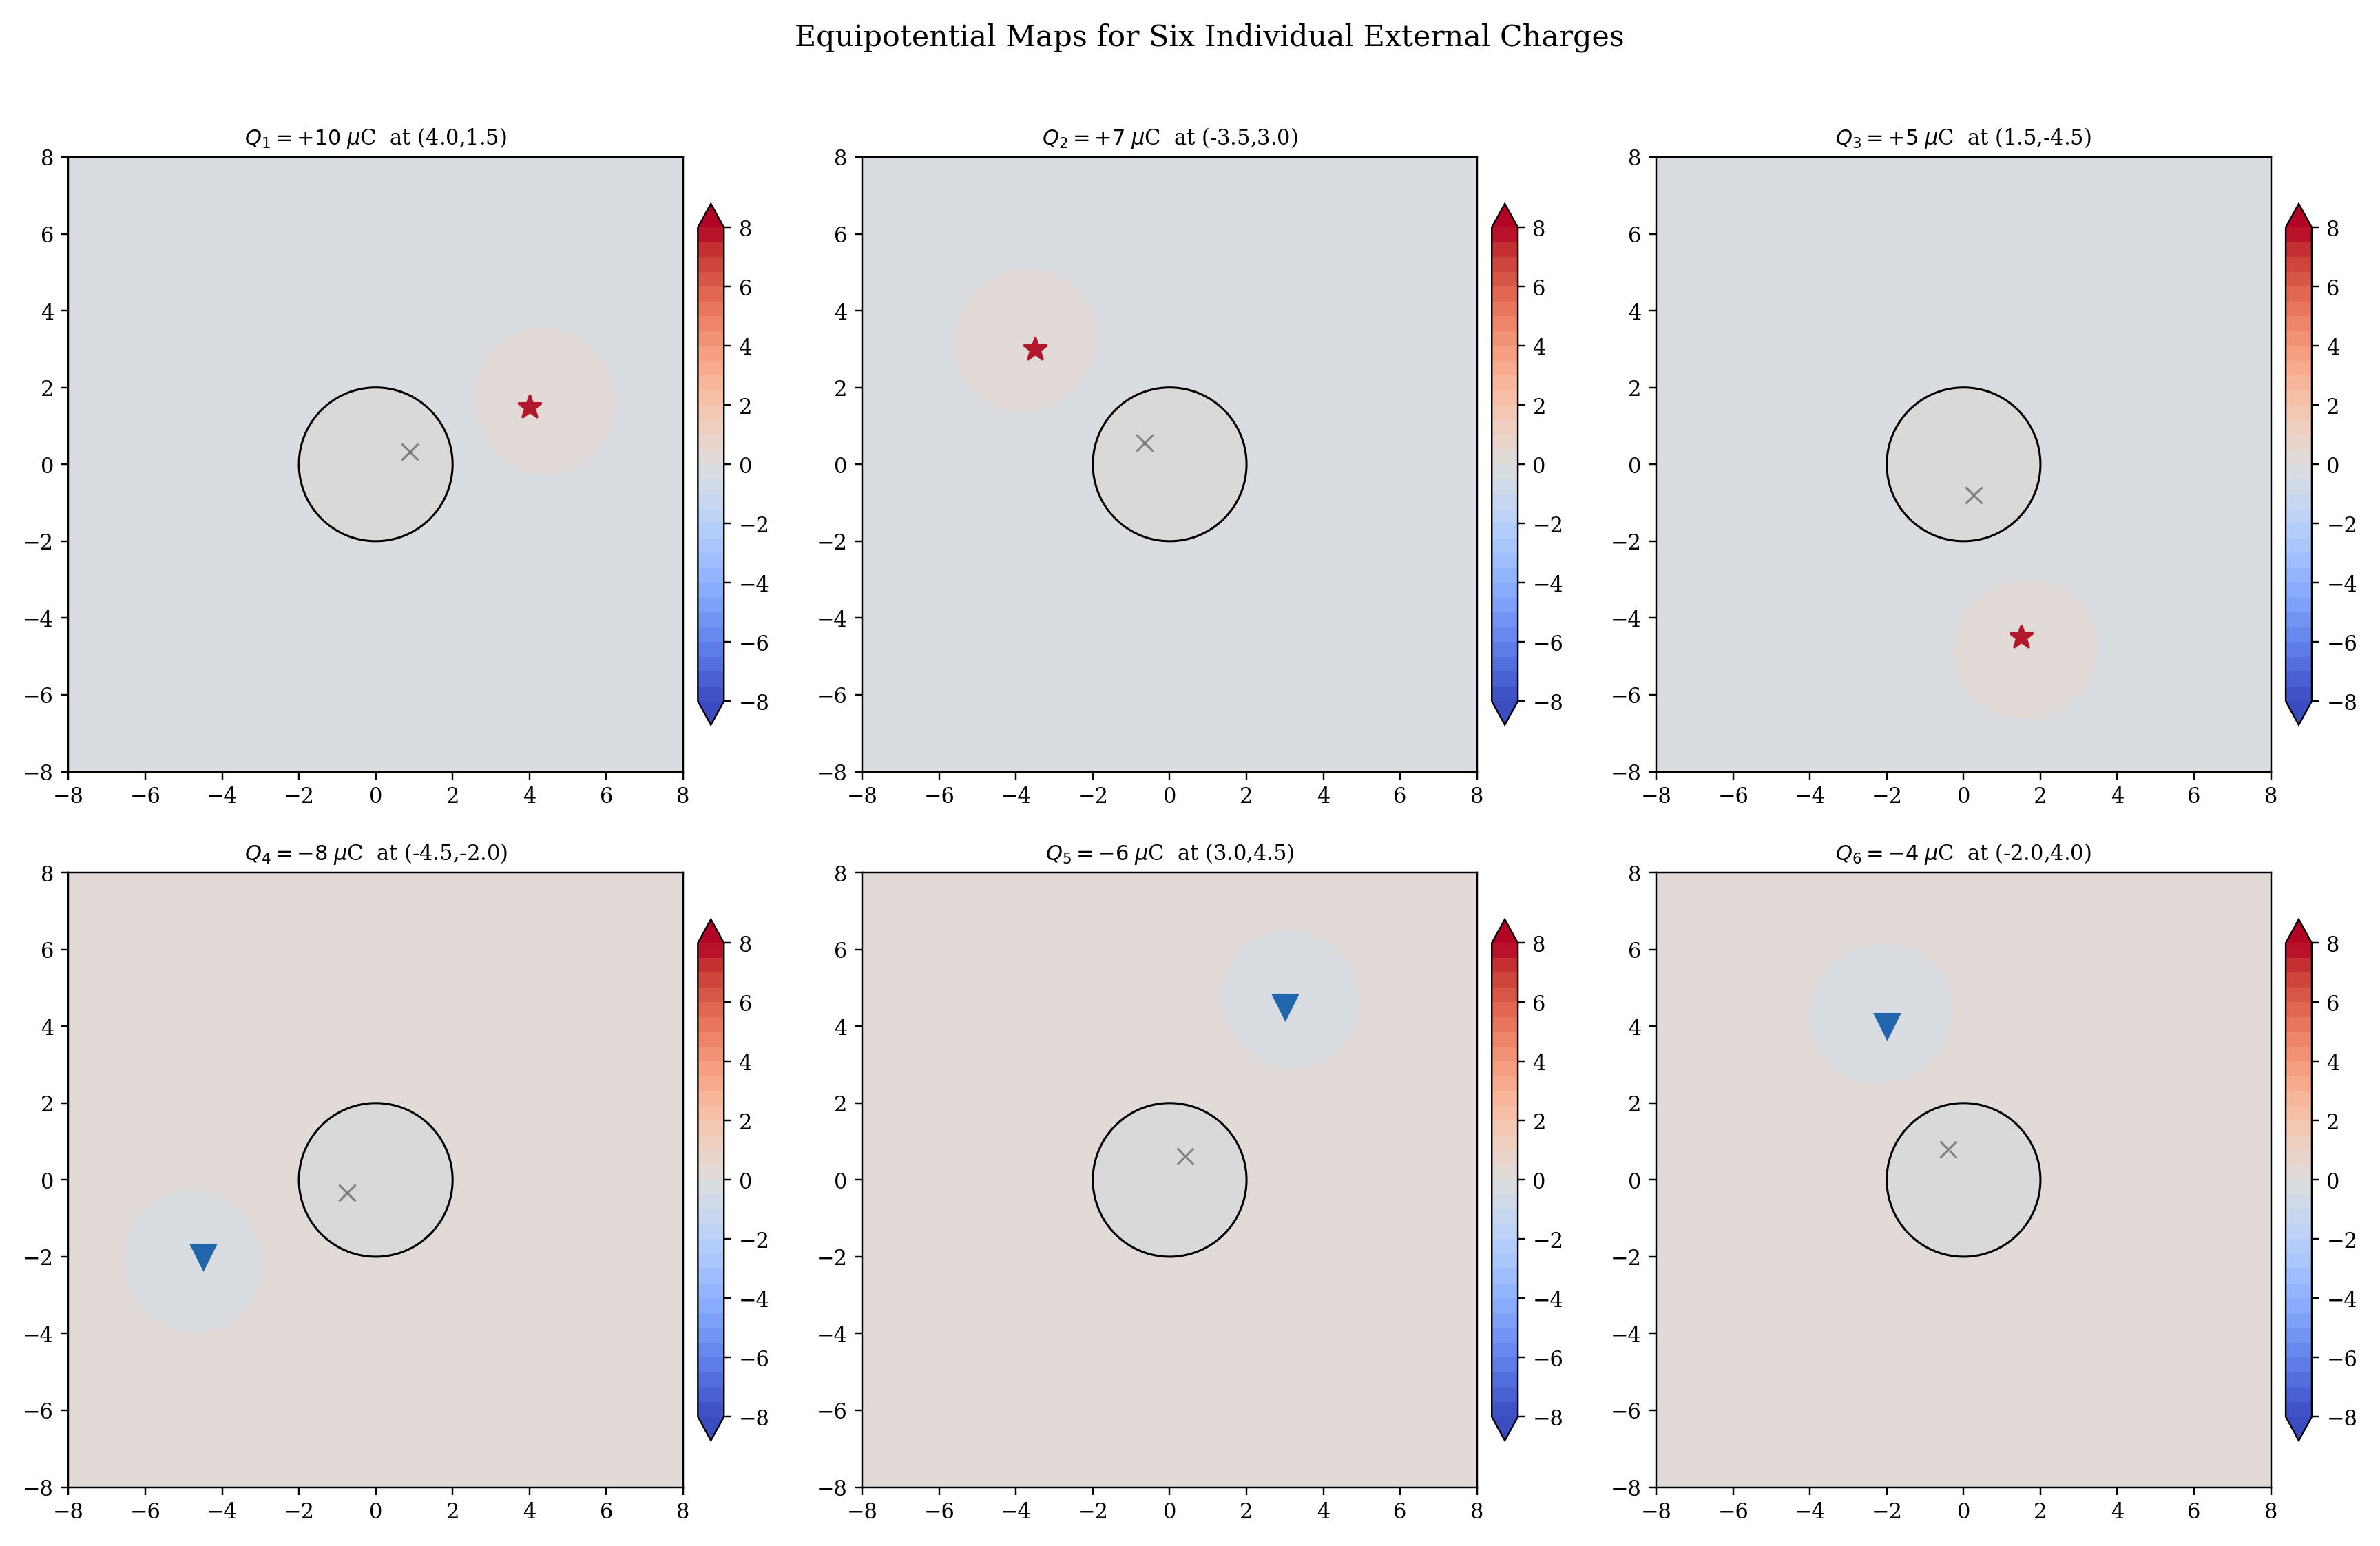
\includegraphics[width=0.95\textwidth]{figures/q2/fig12_multi_individual.png}
\caption{Equipotential maps for six individual external charges, each with its image. The sphere remains at $V=0$ in every case.}
\label{fig:q2_multi_ind}
\end{figure}

\begin{figure}[H]
\centering
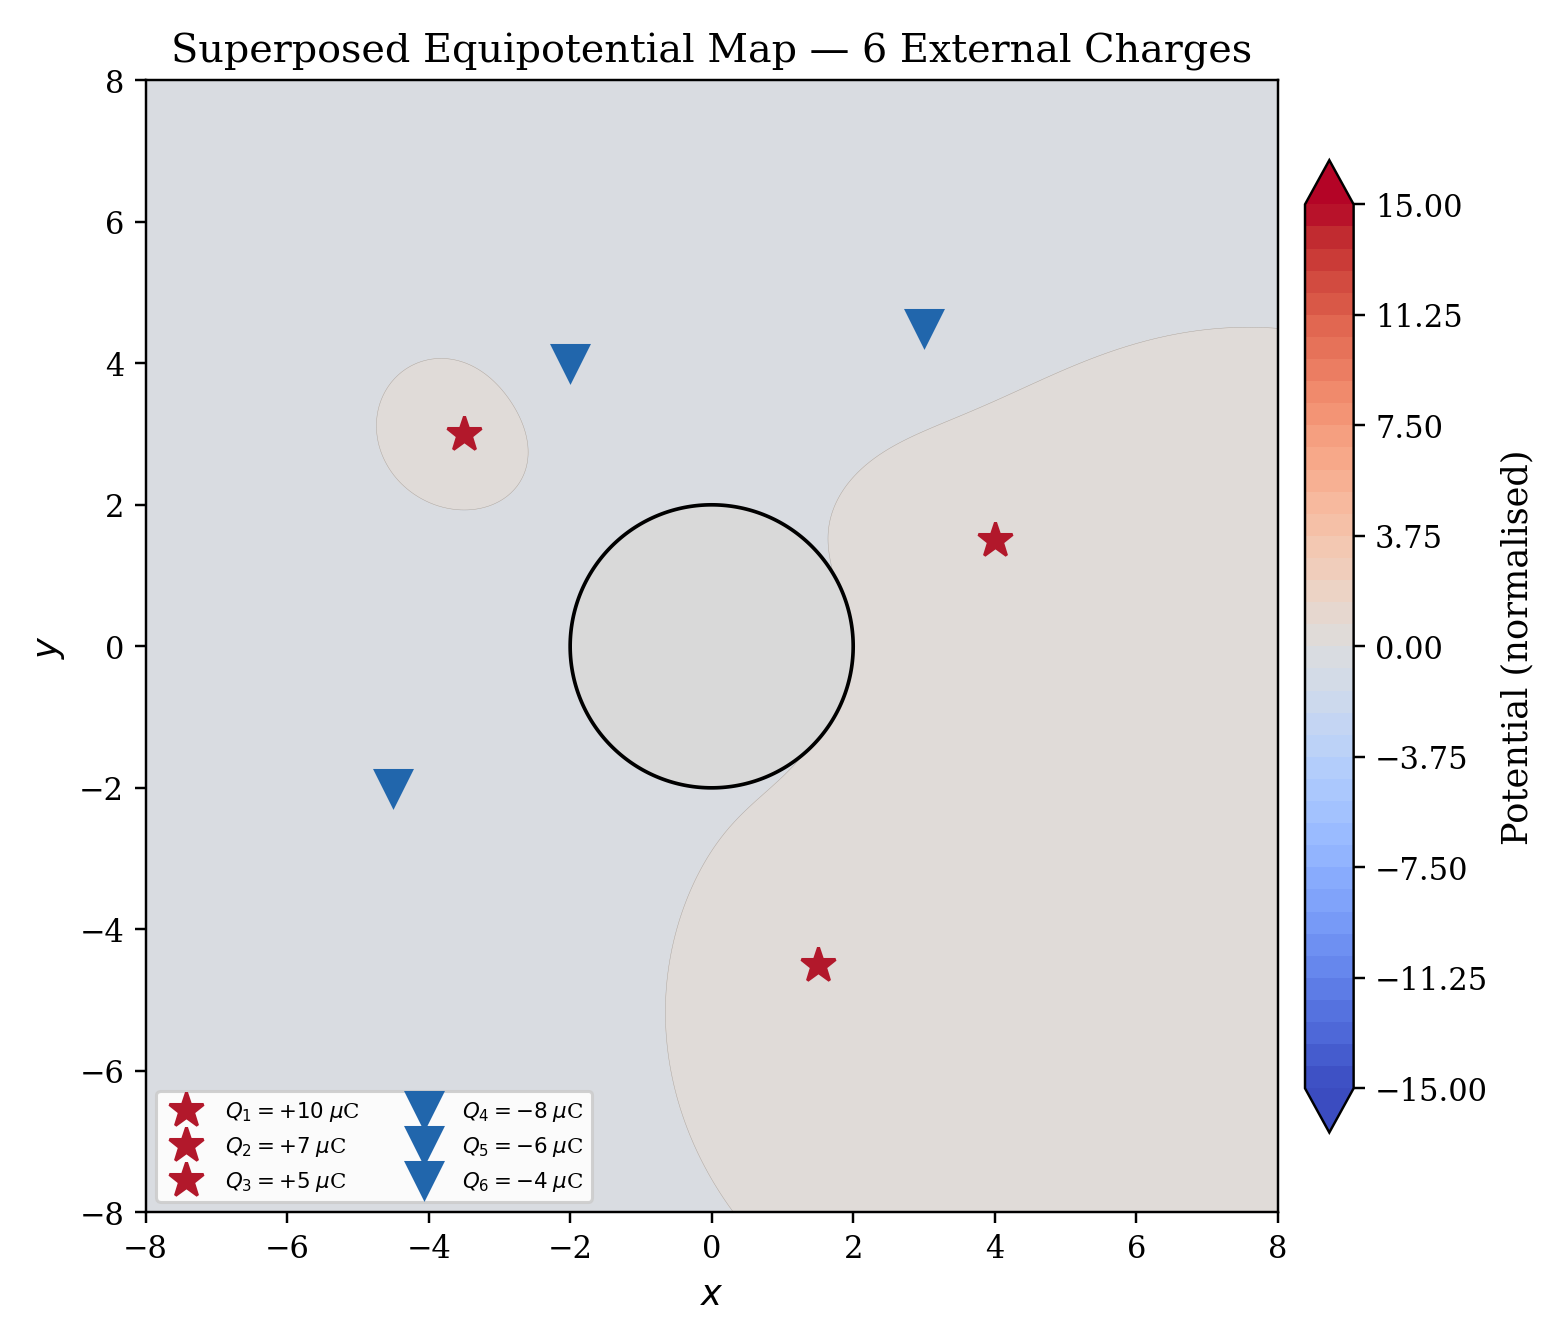
\includegraphics[width=0.82\textwidth]{figures/q2/fig13_multi_combined.png}
\caption{Superposed equipotential map with all six external charges present simultaneously.}
\label{fig:q2_multi_comb}
\end{figure}

\begin{figure}[H]
\centering
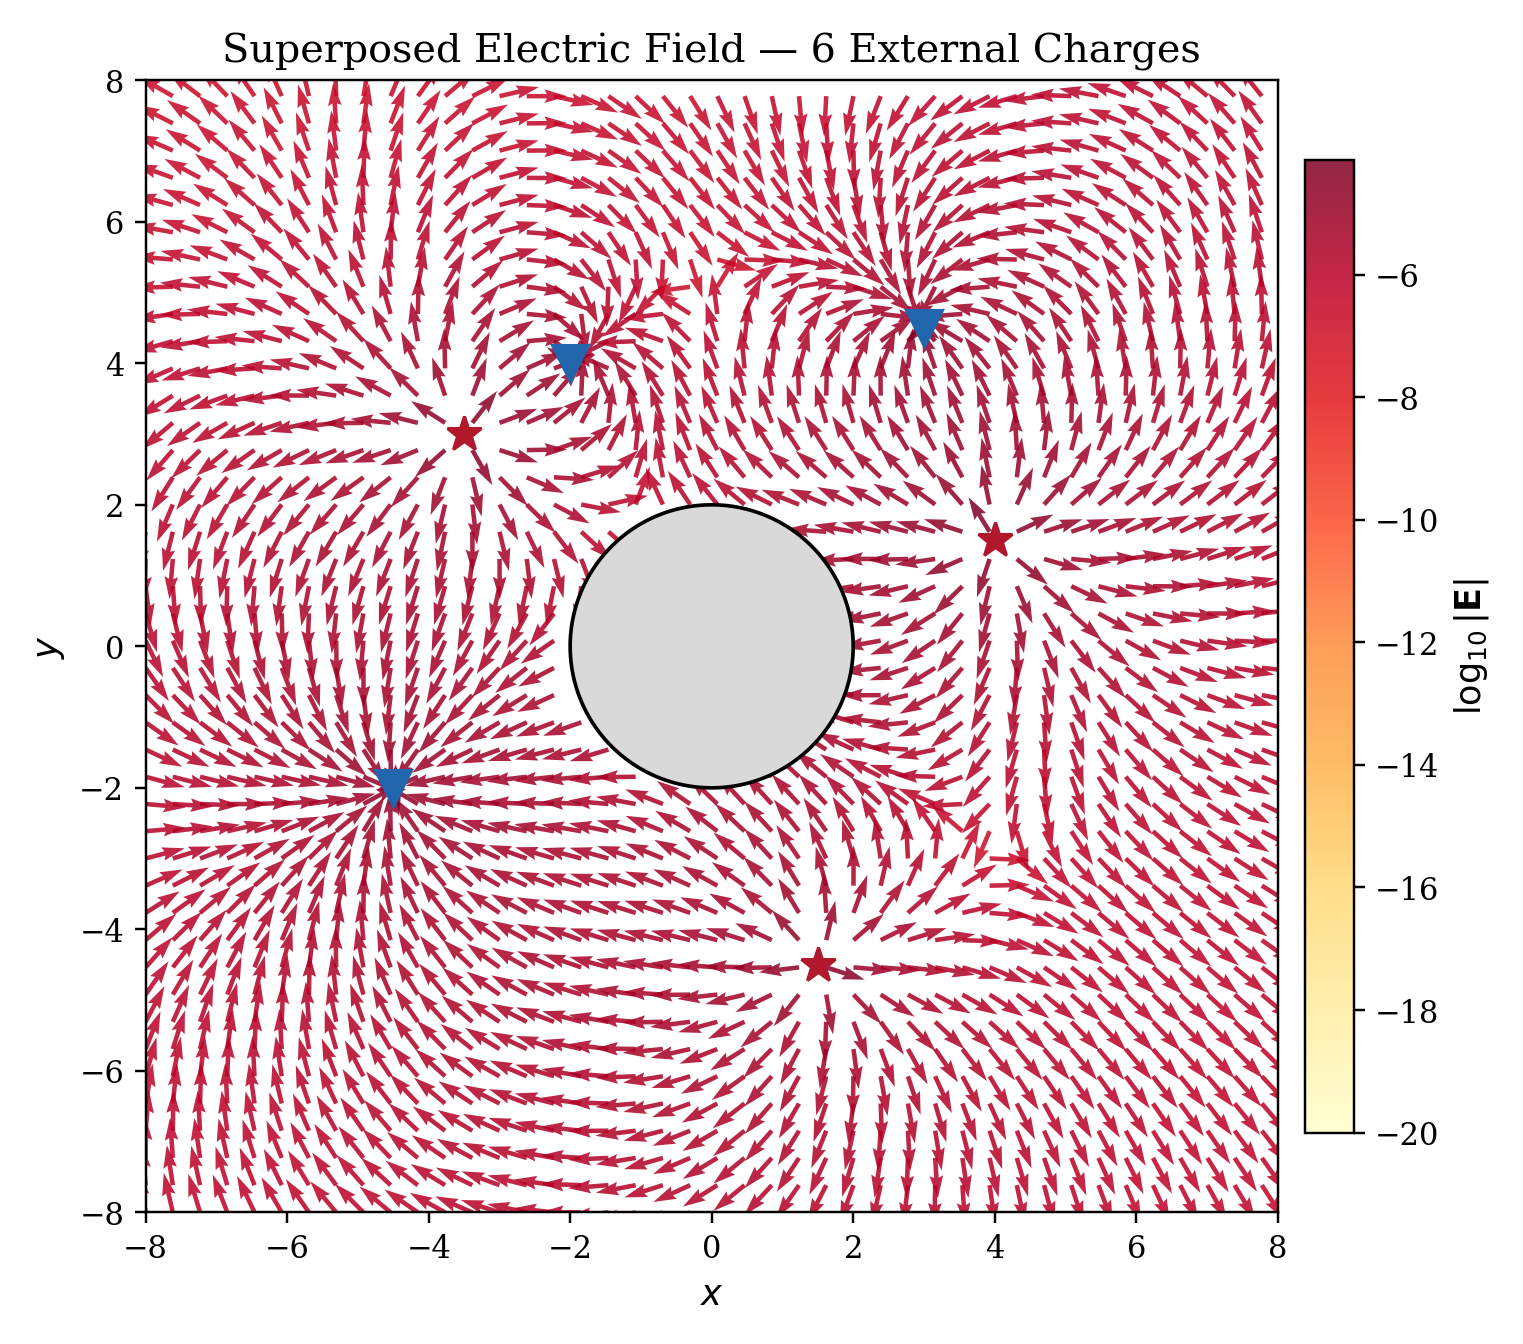
\includegraphics[width=0.82\textwidth]{figures/q2/fig14_multi_field.png}
\caption{Superposed electric field vectors with all six external charges.}
\label{fig:q2_multi_E}
\end{figure}

\begin{figure}[H]
\centering
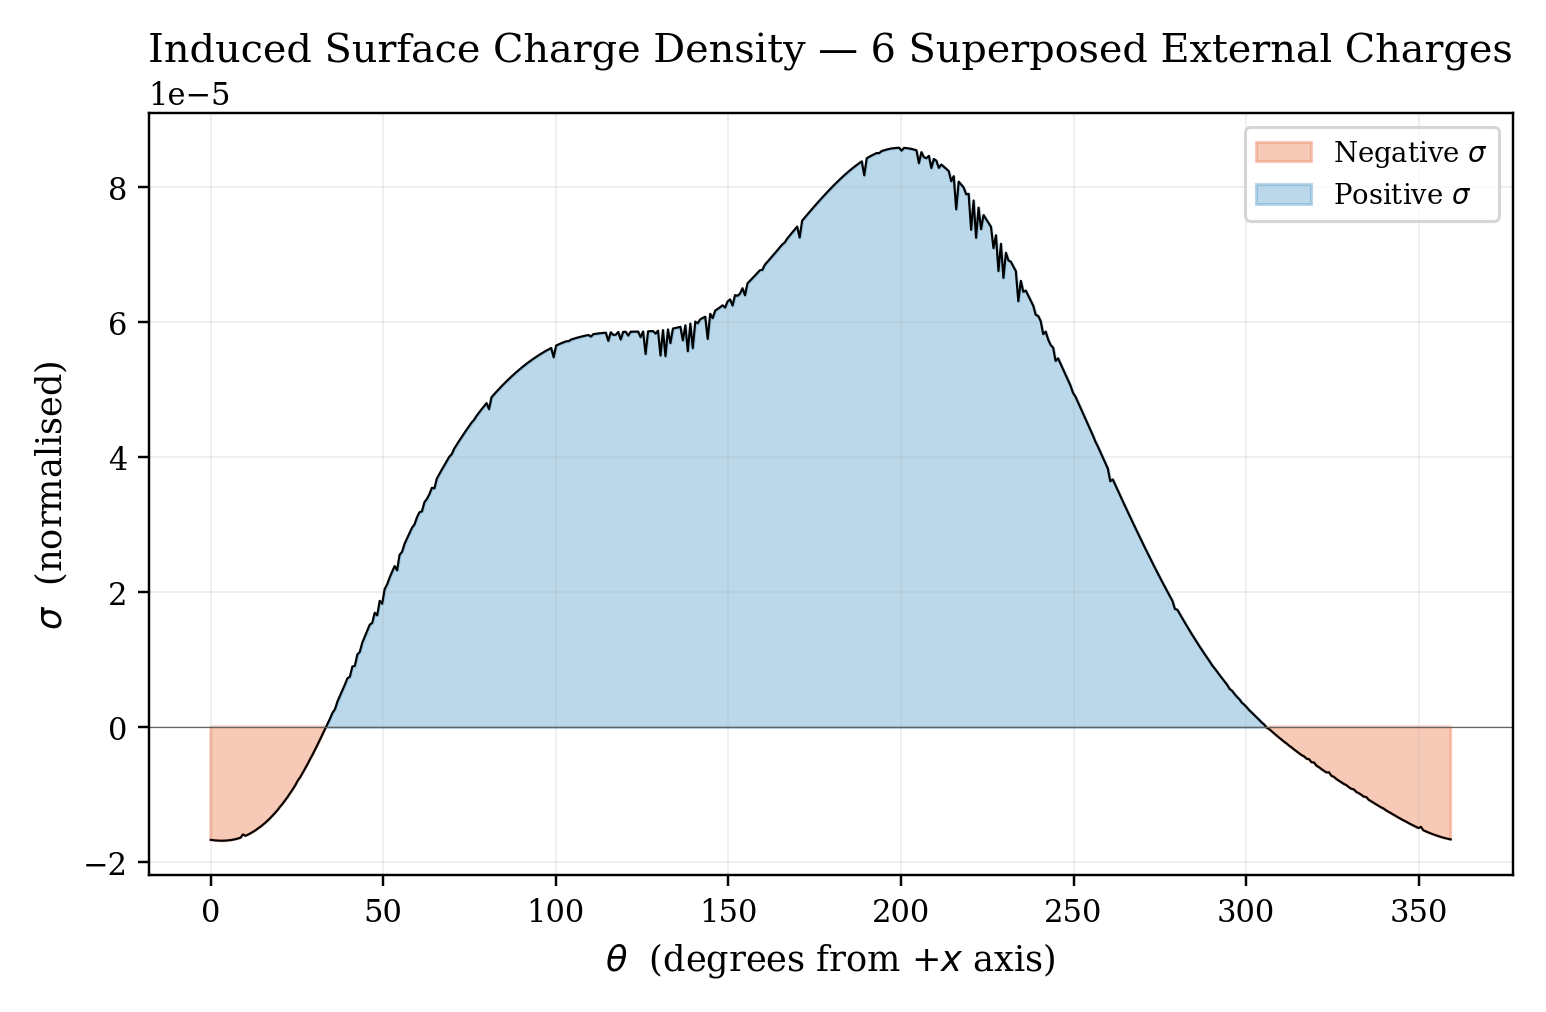
\includegraphics[width=0.82\textwidth]{figures/q2/fig15_multi_sigma.png}
\caption{Induced surface charge density from the superposition of all six external charges. Both positive and negative $\sigma$ regions are present.}
\label{fig:q2_multi_sig}
\end{figure}

\textbf{Observation:} Unlike the single-charge case, $\sigma(\theta)$ is no longer purely negative---it shows both positive and negative regions, reflecting the competing influence of the external charges. The total $\sigma$ is the algebraic sum of the individual contributions, confirming the linearity of the electrostatic problem.

\subsection{Physical Interpretation}
\begin{itemize}[leftmargin=2em]
\item The \textbf{image charge} is a mathematical device that reproduces the correct boundary condition ($V=0$ on the sphere). The real induced charges on the surface produce the same external field as the fictitious image.
\item The \textbf{linearity} of the problem means effects of multiple charges can be summed (\textbf{superposition principle}).
\item As $d \to R$, the image charge approaches the surface, making $\sigma$ increasingly peaked---in the limit, the peak becomes singular.
\end{itemize}

\newpage

% ══════════════════════════════════════════════════════
%  3. LIGHTNING ROD
% ══════════════════════════════════════════════════════
\section{Electric Field Enhancement at a Sharp Conductor (Lightning Rod)}

\subsection{Introduction and Real-World Context}

This simulation demonstrates the operating principle of \textbf{lightning rods}, invented by Benjamin Franklin in the 18th century. A lightning rod is a grounded pointed conductor placed atop a building. During a thunderstorm, the electric field between the charged cloud and the ground is enhanced at the tip of the rod by orders of magnitude relative to the ambient field. Once this local field exceeds the breakdown strength of air (${\approx}3$\,MV/m at sea level), a controlled discharge initiates preferentially at the tip, providing a safe path for current to flow to ground.

\subsection{Problem Formulation}

A $100 \times 100$ grid represents the gap between a ground plane ($V=0$, bottom row) and a charged cloud ($V=100$\,V, top row). The left and right boundaries carry a linear ramp from 0 to 100\,V:
\begin{equation}
V_{\text{side}}(j) = V_{\text{gnd}} + \frac{j}{N-1}\bigl(V_{\text{cloud}} - V_{\text{gnd}}\bigr),
\end{equation}
simulating the ambient uniform field. A grounded conducting needle occupies the centre column from the ground up to row 50 (mid-height), fixed at $V=0$.

\subsection{Numerical Method}

The same four-neighbour Gauss--Seidel scheme \eqref{eq:fivepoint} was used, with all Dirichlet conditions reimposed after each sweep:
\begin{equation}
V_{j,i}^{(k+1)} = \frac{1}{4}\bigl(V_{j,i+1}^{(k)} + V_{j,i-1}^{(k+1)} + V_{j+1,i}^{(k)} + V_{j-1,i}^{(k+1)}\bigr), \quad \text{skipping needle nodes}.
\end{equation}

A convergence check was performed every 500 iterations:
\begin{equation}
\max_{i,j} \bigl|V_{i,j}^{(k)} - V_{i,j}^{(k-500)}\bigr| < 10^{-6}\;\text{V}.
\end{equation}
Convergence was reached at iteration 7\,000.

\subsubsection{Enhancement factor calculation}

The ambient uniform field (without the needle) is:
\begin{equation}
E_0 = \frac{V_{\text{cloud}}}{N-1} = \frac{100}{99} \approx 1.01\;\text{V/grid-unit}.
\end{equation}

The enhancement factor is defined as:
\begin{equation}
\beta_{\text{num}} = \frac{E_{\text{tip}}}{E_0} = \frac{7.608}{1.010} \approx 7.5.
\end{equation}

For comparison, the classical result for a conducting \textbf{prolate spheroid} with semi-major axis $a$ and tip radius $b \ll a$ is:
\begin{equation}
\boxed{\;\beta = \frac{a}{b\,\ln(2a/b)}.\;}
\label{eq:beta_theory}
\end{equation}

Substituting $a = 50$ and $b = 1$ (grid units):
\begin{equation}
\beta_{\text{theory}} = \frac{50}{1 \times \ln(100)} \approx \frac{50}{4.605} \approx 10.9.
\end{equation}

The discrepancy ($7.5$ vs.\ $10.9$) is expected: a single-column needle on a coarse $100 \times 100$ grid is not a perfect spheroid. A finer grid or a more realistic tip geometry would bring the estimates closer.

\subsection{Assumptions}
\begin{enumerate}[leftmargin=2em]
\item \textbf{Electrostatic equilibrium:} Charges have finished moving on the conductors.
\item \textbf{Perfect conductors:} The needle and plates have no resistance; the entire needle is at $V=0$.
\item \textbf{Charge-free air:} No free-floating ions or space charges ($\rho = 0$).
\item \textbf{2D geometry:} The needle is an infinite conducting strip in $z$. A physically sharp needle (tip radius ${\sim}\mu$m) would exhibit far greater enhancement.
\item The linear-ramp side boundary is the simplest condition consistent with the unperturbed uniform field.
\item Air breakdown and space-charge effects are not modelled.
\end{enumerate}

\subsection{Results}

\subsubsection{Potential distribution and field vectors}

\begin{figure}[H]
\centering
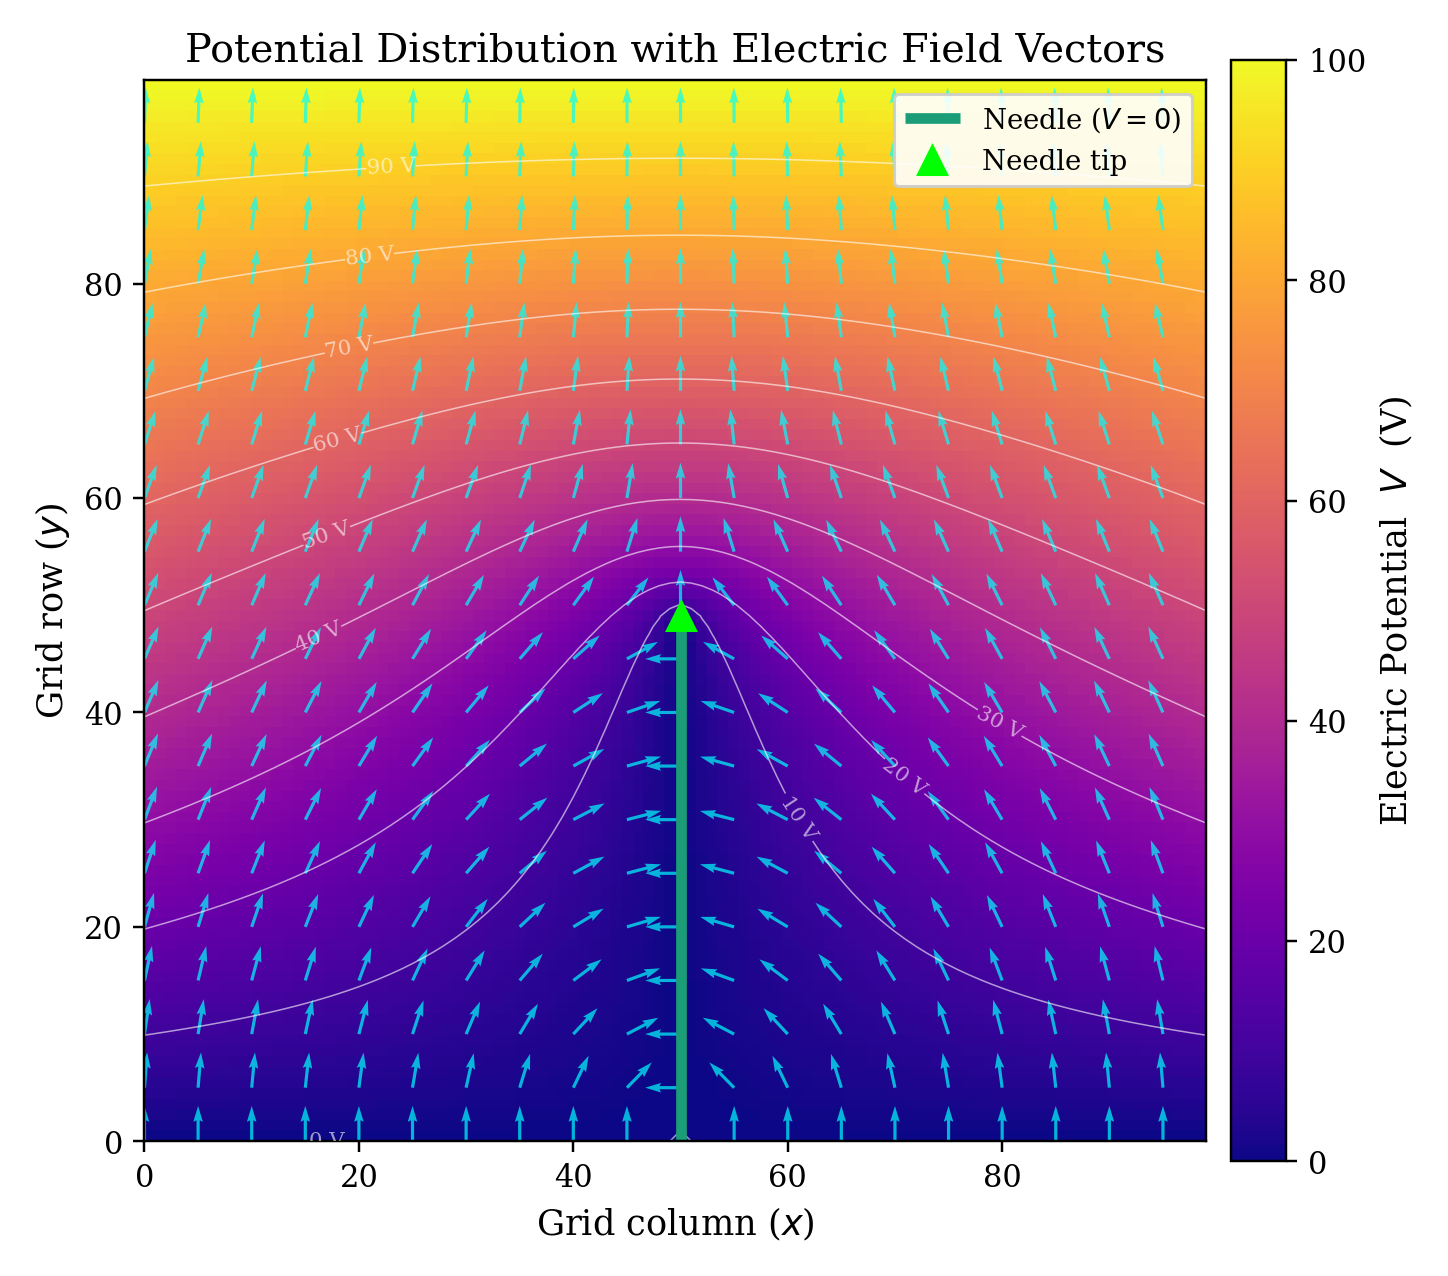
\includegraphics[width=0.82\textwidth]{figures/q3/fig1_potential_field.png}
\caption{Converged potential distribution with white equipotential contours and normalised field-vector arrows. The equipotentials pile up sharply above the needle tip.}
\label{fig:q3_pot}
\end{figure}

\textbf{Observation:} The equipotential lines are horizontal near the top (cloud) but sharply curve and dip around the needle. The crowding right above the tip shows the voltage changing very rapidly over a short distance---the visual signature of field enhancement. The field vectors are ``sucked'' toward the tip.

\subsubsection{Field magnitude ($\log_{10}$ scale)}

\begin{figure}[H]
\centering
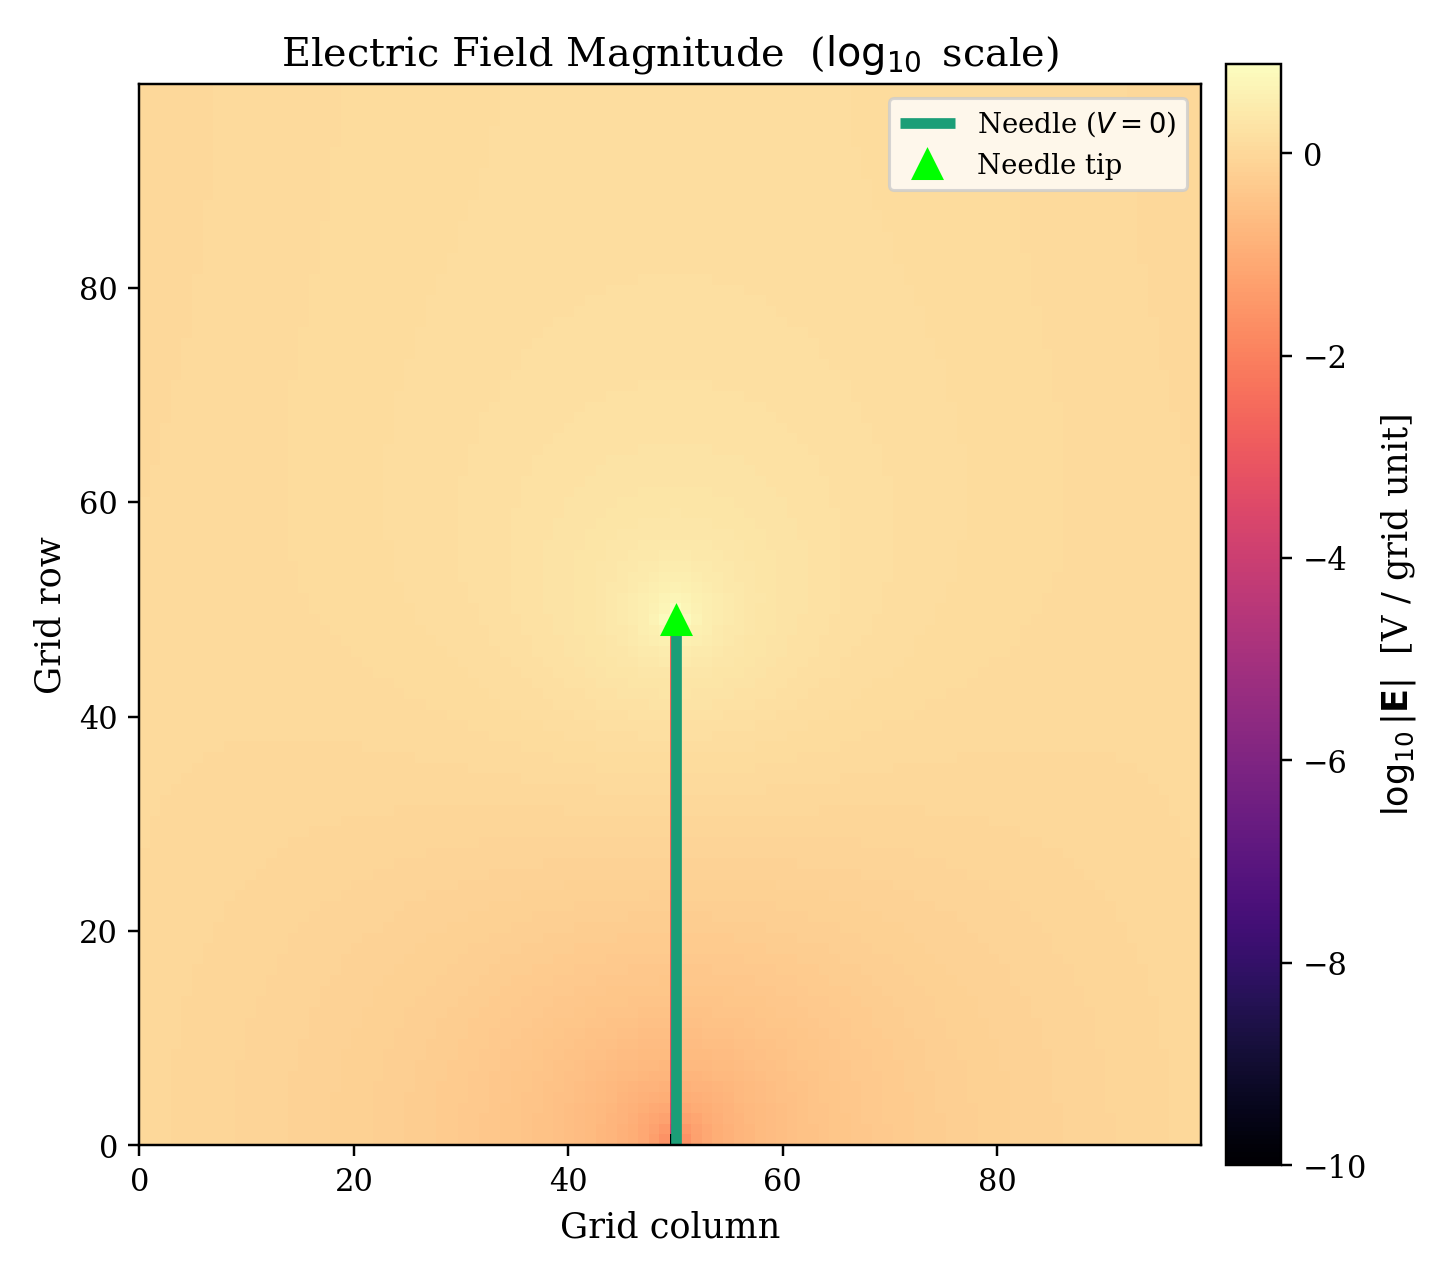
\includegraphics[width=0.82\textwidth]{figures/q3/fig2_field_heatmap.png}
\caption{$\log_{10}|\mathbf{E}|$ heat map. The needle body is dark (zero internal field); the bright spot at the tip is the region of maximum enhancement.}
\label{fig:q3_logE}
\end{figure}

\textbf{Observation:} The logarithmic scale is essential because the dynamic range spans several orders of magnitude. The bright, localised patch above the tip confirms that $|\mathbf{E}|$ is concentrated into a very small region.

\subsubsection{Centre-line field profile}

\begin{figure}[H]
\centering
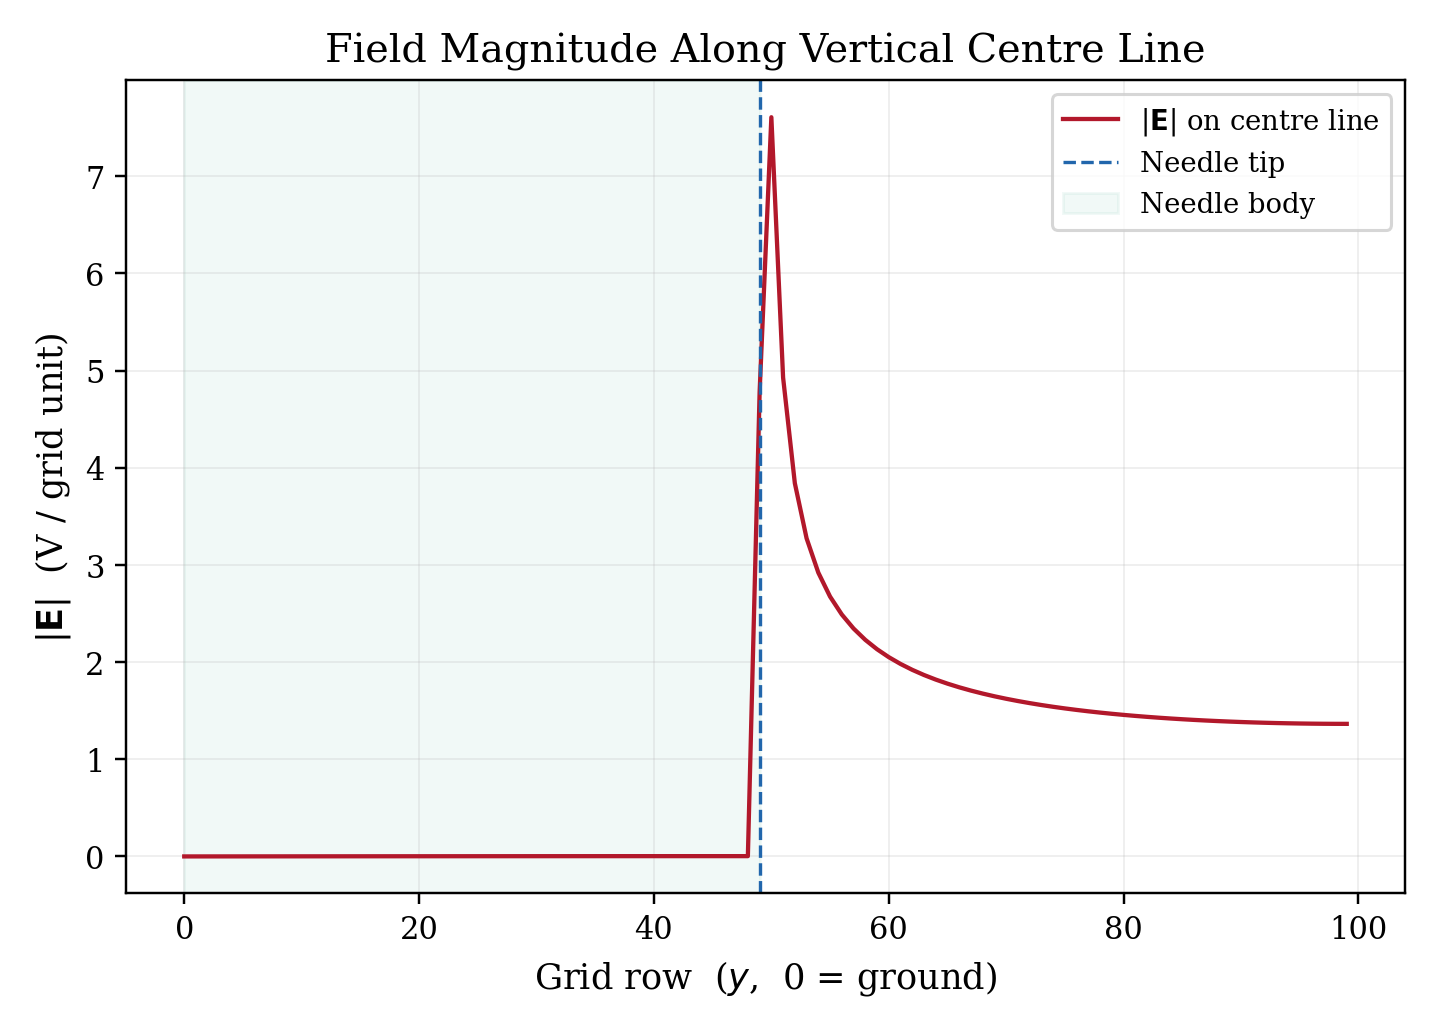
\includegraphics[width=0.82\textwidth]{figures/q3/fig3_centreline_field.png}
\caption{$|\mathbf{E}|$ along the vertical centre line. The cyan band marks the needle body (zero field); the sharp spike above the tip quantifies the enhancement.}
\label{fig:q3_centreline}
\end{figure}

\textbf{Observation:} The field is zero inside the needle (rows 0--50), then shoots up to a peak of ${\approx}7.6$\,V/grid-unit at the tip (row~50), before decaying toward the cloud. This provides the quantitative proof of field enhancement: the peak value is $7.5\times$ the ambient.

\subsubsection{Streamlines}

\begin{figure}[H]
\centering
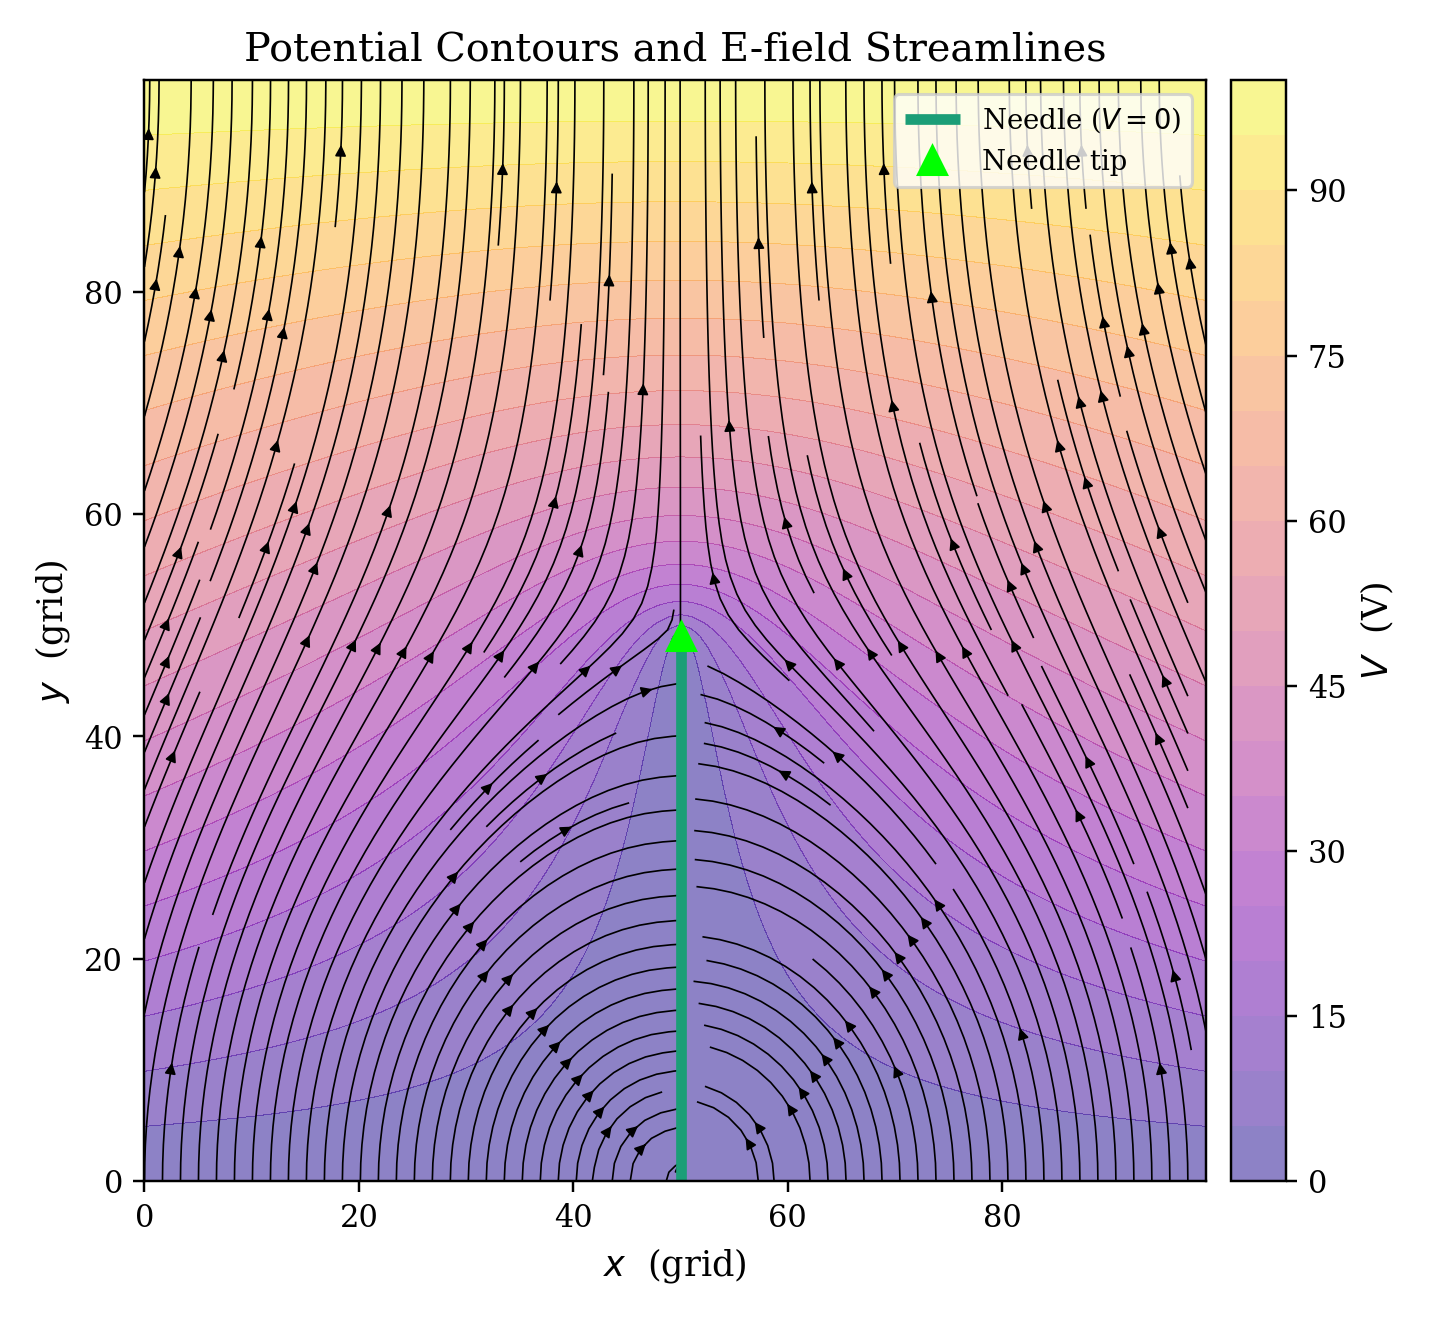
\includegraphics[width=0.82\textwidth]{figures/q3/fig4_streamlines.png}
\caption{Electric-field streamlines overlaid on the potential colour map. Lines from a wide horizontal extent are funnelled into the needle tip.}
\label{fig:q3_stream}
\end{figure}

\textbf{Observation:} Field lines originating far from the needle axis are drawn inward and converge on the tip, concentrating the electric flux into a very small area. This is exactly the mechanism by which a lightning rod initiates a controlled discharge.

\subsubsection{Convergence history}

\begin{figure}[H]
\centering
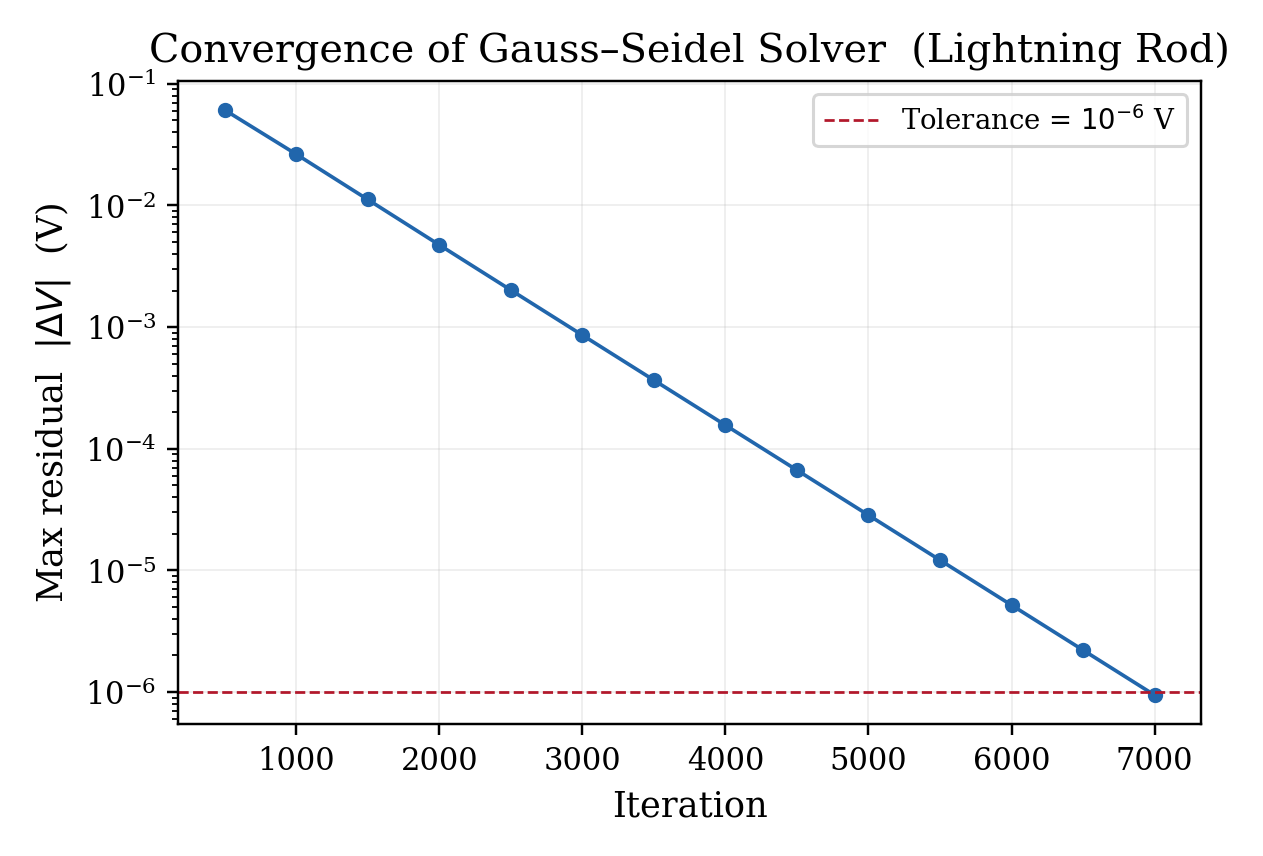
\includegraphics[width=0.55\textwidth]{figures/q3/fig5_convergence.png}
\caption{Convergence history. The maximum residual crosses $10^{-6}$\,V at iteration 7\,000.}
\label{fig:q3_conv}
\end{figure}

\subsection{Physical Interpretation: The Lightning Rod Effect}

The field enhancement at a sharp conductor tip is fundamentally a \textbf{geometric effect}. The conductor forces $V=0$ up to the tip, while the ambient potential at that height would otherwise be ${\sim}50$\,V. This potential difference must be accommodated over the smallest available length scale---the tip radius $b$. Since $E \sim \Delta V / b$, reducing $b$ increases $E$ without bound, as captured by Eq.~\eqref{eq:beta_theory}.

In practical terms, a grounded pointed conductor placed in an external field will develop a surface field at its tip that is orders of magnitude larger than the ambient field. Once this exceeds the dielectric strength of air, corona discharge (and eventually a full arc) initiates preferentially at the tip, providing a controlled path for current to ground. This is the operating principle of the \textbf{Franklin lightning rod}.

\newpage

% ══════════════════════════════════════════════════════
%  4. CONCLUSIONS
% ══════════════════════════════════════════════════════
\section{Conclusions}

Three canonical two-dimensional electrostatic problems were solved numerically, and the results are consistent with analytical expectations in every case.

\subsection{Summary of Key Results}

\begin{table}[H]
\centering
\small
\renewcommand{\arraystretch}{1.3}
\begin{tabular}{lccc}
\toprule
\textbf{Metric} & \textbf{Q1 (Capacitor)} & \textbf{Q2 (Sphere)} & \textbf{Q3 (Lightning Rod)} \\
\midrule
Grid size          & $120 \times 120$ & $300 \times 300$ (MoI) / $201 \times 201$ (iter.) & $100 \times 100$ \\
Iterations         & 5\,000 & --- / 7\,000 & 7\,000 \\
Key validation     & $E_0 \approx 3\,000$ V/m & $V=0$ on sphere ($<10^{-5}$) & $\beta_{\text{num}} = 7.5$ \\
Theory comparison  & $\Delta V / d$ & Linear $\sigma \propto Q$ & $\beta_{\text{theory}} = 10.9$ \\
\bottomrule
\end{tabular}
\caption{Summary of key numerical results across all three problems.}
\end{table}

\subsection{Per-Problem Conclusions}

\textbf{Problem 1:} The parallel-plate capacitor simulation recovered the ideal uniform field of 3\,000\,V/m between the plates, resolved the fringing field at the edges, and correctly predicted the $4{:}1$ field-magnitude jump at a dielectric interface with $\kappa_1/\kappa_2 = 4$. The importance of the initial guess and the convergence advantage of Gauss--Seidel over Jacobi iteration were discussed.

\textbf{Problem 2:} The grounded-sphere simulation confirmed the method of images by verifying $V=0$ on the sphere surface to machine-level precision. The parameter sweeps demonstrated the expected linear scaling of $\sigma$ with $Q$ and the nonlinear sharpening of $\sigma$ as $d \to R$. The iterative Poisson solver produced results consistent with the analytical method, validating both approaches. The multi-charge superposition study demonstrated the linearity of the problem.

\textbf{Problem 3:} The lightning-rod simulation quantified the field-enhancement effect at a sharp conductor tip, obtaining $\beta \approx 7.5$ on the $100 \times 100$ grid, reasonably close to the theoretical spheroid estimate of $\beta \approx 10.9$. The streamline plot provides a compelling illustration of the charge-collection mechanism that underlies lightning protection.

\subsection{Overall Conclusion}

Across all three problems, a consistent theme emerges: the behaviour of electrostatic fields is governed by the interplay between boundary geometry and boundary conditions. The Gauss--Seidel relaxation method proved to be a robust and intuitive numerical tool for solving Laplace's and Poisson's equations in two dimensions. Where analytical solutions exist (method of images for the sphere), they serve as invaluable benchmarks for validating numerical results.

The simulations also highlight key physical phenomena---\emph{fringing fields} at conductor edges, \emph{electrostatic induction} on grounded conductors, and \emph{geometric field enhancement} at sharp tips---that have direct engineering applications: capacitor design, electrostatic shielding, and lightning protection.

\subsection{Possible Extensions}
\begin{itemize}[leftmargin=2em]
\item \textbf{Successive Over-Relaxation (SOR):} Accelerate convergence by using an over-relaxation parameter $\omega \in (1,2)$.
\item \textbf{Adaptive mesh refinement:} Use finer grids near the needle tip or plate edges where gradients are steepest.
\item \textbf{3D modelling:} Extend the sphere problem to a true 3D geometry with the $1/r$ potential.
\item \textbf{Nonlinear effects:} Incorporate air breakdown and corona discharge modelling.
\item \textbf{Multiple dielectric layers:} Model more complex capacitor geometries with graded permittivity.
\end{itemize}

\vspace{1cm}
\noindent\rule{\textwidth}{0.5pt}
\begin{center}
\small\itshape
All simulation code (Python scripts \texttt{q1\_parallel\_plate\_capacitor.py}, \texttt{q2\_point\_charge\_sphere.py}, \texttt{q2\_iterative.py}, \texttt{q2\_multicharge.py}, \texttt{q3\_lightning\_rod.py}, and \texttt{style.py}) is available in the GitHub repository:\\[3mm]
\url{https://github.com/aniket/EE1204-SimAssignment1}\\[2mm]

\end{center}

\end{document}
